%\documentclass[pdflatex,sn-basic]{sn-jnl}% Basic Springer Nature Reference Style/Chemistry Reference Style
\documentclass[mnsc,sglanonrev]{informs4}  % Management Science

%%<additional latex packages if required can be included here>
\usepackage{url}
%\usepackage{graphicx}
\usepackage[T1]{fontenc}
\usepackage[algo2e,linesnumbered,ruled]{algorithm2e} 
%\usepackage{appendix}
\usepackage{tabularx}       % automatic column width
%\usepackage{subfig}        % two aligned subfigures
\usepackage{mathtools}  
\usepackage{amsfonts}       % mathbb
\usepackage{amsmath}        % aligned equations
\usepackage{xfrac}          % slanted fractions
\usepackage{bm}             % bold greeks 
\usepackage [autostyle, english = american]{csquotes} % left and right opening quotes with "
\usepackage{wrapfig}        % text flows around image
\usepackage{array}          % Needed for custom column types
\usepackage{xcolor}
\colorlet{added}{blue!80!black} 
\usepackage{setspace}       % for controlled interline
%\usepackage{lineno}
\usepackage{enumitem}
\usepackage{tikz}           % drawing figures
\usepackage[utf8]{inputenc} % murphy prefers

\usepackage{caption}
\usepackage[labelfont=sf]{subcaption}
\captionsetup{subrefformat=parens,font=footnotesize}
\subcaptionsetup[figure]{textfont=sf,position=bottom}

\allowdisplaybreaks[4]
\interdisplaylinepenalty=100
\raggedbottom  % In preamble; allows uneven page bottoms

%\setstretch{1.25}   % INTERLINE
\OneAndAHalfSpacedXII  % Management Science
\makeatletter
\providecommand{\@currsize}{\normalsize}
\makeatother

% Private macros here (check that there is no clash with the style)
% for authors data

% Natbib setup for author-number style
\usepackage{natbib}
% \bibpunct[, ]{(}{)}{,}{a}{}{,}%
% \def\bibfont{\small}%
% \def\bibsep{\smallskipamount}%
% \def\bibhang{24pt}%
% \def\newblock{\ }%
% \def\BIBand{and}%

% Redefine X column in tabularx to center the content
\newcolumntype{C}{>{\centering\arraybackslash}X}

%% the following for reducing space around figures
\setlength{\intextsep}{4pt}
\setlength{\textfloatsep}{4pt}
\setlength{\textfloatsep}{4.0pt plus 2.0pt minus 2.0pt}
%\captionsetup{belowskip=0pt}
\setlist[itemize]{noitemsep,nolistsep}

\MakeOuterQuote{"}
\def\UrlFont{\rmfamily}
\newtheorem{proposition}{Proposition}
\theoremstyle{remark}\newtheorem{remark}{Remark}
%%\unnumbered% uncomment this for unnumbered level heads

\MANUSCRIPTNO{MNSC-0001-2024.00} % Management Science

\begin{document}
\let\WriteBookmarks\relax
\def\floatpagepagefraction{1}
\def\textpagefraction{.001}
	
% Reduce space before and after align
\setlength{\abovedisplayskip}{2pt plus 2pt minus 4pt}
\setlength{\belowdisplayskip}{2pt plus 2pt minus 4pt}
\setlength{\abovedisplayshortskip}{0pt}
\setlength{\belowdisplayshortskip}{0pt}

% Management Science section
\RUNAUTHOR{Fenga ans Maniezzo}
\RUNTITLE{Bootstrap Enhanced Scenario Optimization}
\TITLE{Bootstrap Enhanced Scenario Optimization, a Case Study in City Logistics}
\ARTICLEAUTHORS{%
%\AUTHOR{John Doe,\textsuperscript{a} Jane Smith,\textsuperscript{b}}
%\AFF{\textsuperscript{a}Department of Industrial Engineering, University of XYZ, \EMAIL{john.doe@xyz.edu; \textsuperscript{b}Department of Computer Science, University of ABC, \EMAIL{jane.smith@abc.edu}} 
\AUTHOR{Livio Fenga}
\AFF{Center for Simulation, Analytics and Modelling,
University of Exeter, \EMAIL{L.Fenga@exeter.ac.uk}}

\AUTHOR{Vittorio Maniezzo}
\AFF{Department of Computer Science,
University of Bologna, \EMAIL{vittorio.maniezzo@unibo.it}}
% Enter all authors
} % end of the block

% Springer section
%\title[Article Title]{Bootstrap Enhanced Scenario Optimization, a Case Study in City Logistics}
%
%\author[1]{\fnm{Livio} \sur{Fenga}}\email{L.Fenga@exeter.ac.uk}
%\equalcont{These authors contributed equally to this work.}
%
%\author*[2]{\fnm{Vittorio} \sur{Maniezzo}}\email{vittorio.maniezzo@unibo.it}
%\equalcont{These authors contributed equally to this work.}
%
%\affil[1]{\orgdiv{Center for Simulation, Analytics and Modelling}, \orgname{University of Exeter}, \orgaddress{\city{Exeter}, \postcode{EX4 4PU}, \country{UK}}}
%
%\affil*[2]{\orgdiv{Department of Computer Science}, \orgname{University of Bologna}, \orgaddress{\city{Cesena}, \postcode{47521}, \country{Italy}}}


%\abstract{
\ABSTRACT{
We propose a data‑driven robust optimization framework for logistics, where bootstrapped forecasts define the ambiguity set to achieve improved worst‑case performance.\
We introduce the Bootstrap Enhanced Scenario Optimization (BESO) framework, a novel methodology for prescriptive analytics under uncertainty. BESO addresses the challenge of generating reliable demand scenarios from volatile, short, and non-stationary time series data. The core innovation lies in delegating the modeling of uncertainties to the Maximum Entropy Bootstrap (MEB) integrated with bagging, a technique that preserves the complex autocorrelation structure of empirical time series forecasts, enabling the generation of statistically coherent scenarios. We further extend MEB through an objective-augmented formulation that incorporates downstream recourse elements into the resampling mechanism. These statistically rich scenarios are then integrated into a deterministic equivalent model to derive accountable and optimized prescriptions. We demonstrate the framework's power using a real-world case study in tactical inventory allocation. Our findings, also validated against an extensive set of artificial benchmark instances, demonstrate the effectiveness of MEB-enhanced forecasting in optimization. BESO establishes a new, generalizable paradigm for robust decision-making derived from noisy univariate data series.}

\FUNDING{This research was supported by [grant number, funding agency].}
% Keywords
\KEYWORDS{Stochastic programming, Distributionally Robust Optimization, Forecasting, Maximum Entropy Bootstrap, Two-echelon logistics}

%%\pacs[JEL Classification]{D8, H51}

%%\pacs[MSC Classification]{35A01, 65L10, 65L12, 65L20, 65L70}

\maketitle

\section{Introduction} \label{Sec:intro}

Decision-making under uncertainty is a pervasive challenge in operations research, particularly in complex systems such as logistics networks. Scenario-based optimization has long been used to address this challenge by capturing the variability of future events through a finite set of possible outcomes. However, the reliability of such methods depends heavily on how accurately these scenarios represent the underlying stochastic processes.

In this paper, we propose a novel method —- {\em Bootstrap Enhanced Scenario Optimization} (BESO) —- that integrates bootstrap-based forecasting with scenario-based linear optimization to enhance the robustness and realism of stochastic modeling. The approach can be framed within the Distributionally Robust Optimization (DRO) paradigm; however, unlike mainstream moment- or ambiguity-set-based formulations, it leverages statistical models fitted to empirical data to generate optimization-ready scenarios.

BESO introduces a twofold, decision-aware extension of the Maximum Entropy Bootstrap (MEB). First, the bootstrap objective is augmented with optimization cost components, allowing scenario generation to internalize downstream decision criteria. Second, we explicitly account for the effect of bootstrap-set cardinality on the resulting optimization outcomes, recognizing scenario size as a structural parameter shaping the effective ambiguity set. Together, these mechanisms create a feedback loop between the optimization model and the statistical resampling phase: the ambiguity set remains statistically coherent while its geometry and dispersion are partially shaped by optimization-relevant considerations. The framework is particularly suited to predictive settings where model uncertainty dominates innovation noise, as it is typically the case of short or non-stationary series.

The resulting data-driven methodology for empirically estimating the distribution of stochastic variables and embedding it in scenario generation for robust and stochastic optimization may offer significant advantages over standard distribution-aware approaches. Traditional methods often rely on strong assumptions about the underlying probability distribution — typically normality or other parametric forms — which may not accurately reflect the true behavior of real-world uncertainties. In contrast, data-driven techniques directly leverage historical or observed data to construct empirical distributions, capturing nuances such as asymmetry, multimodality, or heavy tails that standard models might overlook. This increased fidelity can lead to more realistic and effective scenario generation, improving both the robustness and relevance of the resulting optimization solutions. Furthermore, by adapting to the structure present in the data, data-driven approaches are naturally more flexible and can better accommodate nonstationarities or structural changes in the stochastic environment, providing better alignment with real operational environments.

To demonstrate the practical value and performance of BESO, we apply it to a real-world two-echelon logistics network problem. In this setting, uncertain outbound freight demands must be satisfied across multiple depots. By using BESO to define demand scenarios and solve for optimal allocation decisions and related inventory requests, we show how the method improves the solution robustness compared to conventional techniques, while remaining conceptually transparent, computationally efficient and straightforward to implement.

The remainder of the paper is structured as follows: Section \ref{Sec:literature} reviews previous works related to the different research areas intersected by this study. Section \ref{Sec:testcase} describes the case study that motivated our research. Section \ref{Sec:BESOtheory} presents the BESO methodology in detail. Section \ref{Sec:results} discusses the computational results, and Section \ref{Sec:conclusions} concludes with key insights and future research directions.

\section{Literature review} \label{Sec:literature}

The paper intersects different research threads, both in terms of the theoretical contribution and the application use case.

\subsection{Predictive Prescriptions and Distributionally Robust Optimization}

Stochastic programming has long served as a fundamental framework for modeling decision-making under uncertainty, primarily through expected-value models and recourse formulations \citep{D55,B55}. As the field matured, methods evolved to address model robustness. Robust optimization \citep{BS04} proposes a deterministic reformulation considering worst-case outcomes within a defined uncertainty set. A major development is {\it Distributionally Robust Optimization} (DRO), which seeks decisions that are robust against the worst-case probability distribution of the uncertain parameters within a prescribed {\it ambiguity set} \citep{DY10}.

The ambiguity set ($\mathcal{U}$) in DRO is a carefully constructed family of probability distributions that is assumed to contain the true, but unknown, distribution of the uncertain parameters. The core idea is to optimize the worst-case expected performance over all distributions within this set, thereby providing robustness against distributional uncertainty. Different DRO methodologies differ primarily in the way this ambiguity set is defined. \citet{DY10} propose ambiguity sets characterized by known moment information, such as bounds on the mean vector and covariance matrix of the uncertain parameters. \citet{BTGN13} instead consider ambiguity in probability distributions characterized through $\phi$-divergence-based uncertainty regions, which can be constructed as statistical confidence regions around estimated probability vectors. More recently, \citet{EK18} define the ambiguity set as a Wasserstein ball around the empirical distribution, obtaining tractable convex reformulations while providing finite-sample performance guarantees. Despite their differences, these approaches share the common characteristic that the ambiguity set is designed independently of the forecasting process that generates the uncertain parameters.

A primary technique for applying both stochastic programming and DRO is {\it Scenario-Based Optimization}. This approach discretizes the continuous probability distribution of uncertain parameters into a finite set of representative scenarios. The {\it Sample Average Approximation} (SAA) method is a cornerstone of this paradigm \citep{SH98}, approximating the unknown distribution by the empirical distribution obtained from a sample of independent and identically distributed realizations. Extending this idea, \citet{BK19} replace the uniform scenario weights of SAA with covariate-dependent weights derived from nonparametric learning methods, yielding predictive prescriptions that approximate the conditional distribution of the uncertain parameters given observed side information.

The integration of forecasting and scenario-based optimization---often referred to as {\it predict-then-optimize}---has recently attracted considerable attention. The traditional workflow follows a two-stage paradigm in which a forecasting model (e.g., SARIMA, GARCH, or LSTM) first predicts future uncertain parameters, after which a separate scenario generation phase constructs the optimization input from the predictive distribution. This sequential approach has been questioned because prediction errors that are statistically small may nevertheless induce substantial degradation in the quality of the downstream decision. To address this limitation, \citet{EG22} propose the {\it Smart Predict-then-Optimize} (SPO) framework, in which the prediction model is trained using a loss function that measures the resulting decision regret rather than conventional prediction error. Consequently, the learned predictor is optimized for its usefulness to the downstream optimization problem rather than solely for predictive accuracy. Unlike DRO approaches, however, SPO does not model uncertainty through ambiguity sets nor optimize against worst-case probability distributions, but remains an empirical risk minimization framework with a decision-aware loss.

Unlike these traditional DRO and predict-then-optimize approaches, our work introduces a novel framework that fundamentally links the statistical modeling of input data to the generation of the uncertainty set. Our {\it Bootstrap Enhanced Scenario Optimization} (BESO) framework leverages bootstrapped time series to generate future scenarios. This approach is conceptually aligned with DRO, as it seeks robustness across a set of statistically plausible distributions. However, rather than specifying the ambiguity set {\it a priori} through moment constraints, statistical divergences, or Wasserstein distances, BESO induces it directly from the bootstrap distribution generated by the Maximum Entropy Bootstrap (MEB), preserving the autocorrelation structure, non-stationarity, and other empirical characteristics of the historical time series. Moreover, scenarios are not generated as a post-processing step following forecasting, but emerge directly from the statistical model itself. Finally, we extend the MEB objective function by incorporating a downstream optimization component, thereby making the forecasting process explicitly aware of the optimization objective while simultaneously preserving the distributional robustness inherent in the bootstrap-generated scenario set. In this sense, our approach combines the complementary strengths of DRO, which emphasizes robustness to distributional uncertainty, and decision-aware learning methods such as SPO, which emphasize the quality of downstream decisions.

\subsection{2-echelon logistics networks}

Multi-echelon inventory management is a supply chain control strategy that coordinates inventory across multiple levels, called "echelons," of the chain \citep{Clark60}. The objective is to optimize inventory and routing costs across all levels of the supply chain rather than addressing each level in isolation. The literature on this strategy has expanded significantly, covering various aspects such as inventory control policies, replenishment strategies, and inventory risk management.

The successful implementation of effective management policies hinges on sound forecasting and optimization processes. Specifically, in the context of 2-echelon logistics, prescriptions grounded in predictive analytics are essential for refining demand forecasting, inventory allocation, and transportation planning \citep{A01}. Considerable attention has been paid to demand forecasting \citep{Ma15,Shenstone01}, however, precise demand forecasting, especially within the context of dynamic retail environments characterized by fluctuating trends and seasonal variations, remains a significant obstacle. Multi-echelon demand forecasting commonly incorporates a variety of models that frequently rely on assumptions of stationarity and specific parametric distributional characteristics that are often violated in dynamic retail environments characterized by short-horizon, non-stationary demand series, leading to model mismatch and suboptimal prescriptions.

The application of prescriptive analytics in 2-echelon logistics systems thus faces a critical challenge: how to robustly model the underlying uncertainty to support efficient management decision processes. Most documented multi-echelon inventory policies in the literature rely on instances with generic demand, often generated according to parametric distributions \citep{Escorcia20}. Our work addresses this methodological gap.

By introducing the BESO framework, we provide a statistically-grounded approach to tactical logistics planning. BESO leverages the MEB to generate demand scenarios that accurately preserve the complex autocorrelation and non-stationary structure of empirical demand data. This novel method directly counters the limitations of traditional approaches that fail to capture the nuances of real-world volatility, enabling the distribution centers (DCs) to update their market forecast and anticipate the structural attributes of the model, ultimately providing valuable management insights \citep{P16}. We demonstrate this capability using a comprehensive real-world case study where all instance elements, from demand series to network configurations, are derived from actual records. This application provides a validation of how BESO improves both solution robustness and operational efficiency in multi-echelon inventory management.

\section{The 2-echelon test case} \label{Sec:testcase}

The test case, makes use of data that comes from an LSRT company that manages multiple retail stores in a large city in northern Italy, and was originally proposed in \citet{MZ23} for a different application that did not involve stochastic models. In this case, 52 stores provided aggregate sales time series data spanning at least 45 months prior to the forecast period, which is set at a three-month horizon, as detailed in the following. Each store maintains a small inventory, replenished by deliveries from one of four different distribution centers (DCs) in the area. The products are categorized into three lines: fresh, dry, and household. In this context, the focus has been exclusively on the logistics of dry and household goods, including product categories ranging from personal care items to basic electronics, from household goods to holiday decorations. For these product lines, DCs are required to maintain an aggregate inventory sufficient to cover a demand for a period of two weeks.

The supply chain consists of a large distribution center (DC) in the northern suburbs of the city, a smaller DC in the south, and two small satellite facilities closer to the city center. The satellites have limited storage capacity, but they offer lower-cost and more timely service to the majority of the city's stores.  Notably, the three smaller DCs are owned by the company, whereas the fourth DC is situated in a leased facility.
We are concerned only with the DC-to-store part of the network. Each store must be allocated to a DC so that the total monthly demand assigned to it does not exceed its effective monthly service capacity. This capacity is derived from the available storage space under the two-week inventory coverage requirement, accounting also for any local handling limits. It is assumed that the global handling and transportation capacities will always be sufficient to meet the aggregated demand. Both storage capacities and requests are quantified in terms of pallets, with no further granularity at this level. At the level of abstraction of interest, the cost of servicing a store from a DC is assessed based on the travel time required to transport goods between the two entities, independently of pallet volume. The alignment of transportation and rental costs was preprocessed prior to our involvement.

The ultimate goal of the analysis is to determine how much space to rent during the next peak demand period, the Christmas season, where the floorspace to rent is a direct function of the number of pallet to handle. To achieve this, we optimize the allocation of stores to DCs, taking into account transportation, handling and storage costs, optimizing the floorspace to rent or keeping it as an external parameter to be set by what-if simulation runs.

Another requirement characterizes the problem we are addressing: large stores located near small DCs often lead to rapid saturation of the capacity of central DCs. This forces nearby stores to be served by comparatively distant DCs. Therefore, it has been proposed to allow tentative split service for certain selected stores to facilitate further what-if analysis. The problem we address thus involves a parametric number of possible assignments for each store, where which store should be allowed multiple (double) assignments is an input parameter, not a decision variable.  

Because a single store's demand in some simulations can be served by more than one DC, the core optimization problem is a split allocation problem (SAP). This variant of the basic allocation problem has already received attention in the optimization literature, mainly in the context of survivable communication network design \citep{MKE75}, and more generally as the splittable capacitated multiple allocation hub location problems \citep{M05}. It finds applications in fiber optic access networks \citep{KLH11}, split delivery routing \citep{DT89}, and even in school timetabling \citep{BBL07}. We use the same underlying dataset as \citet{ZHHY21}, where stochastic aspects were not modelled.
The SAP mathematical model we use is a direct extension of the standard model for allocation problems. In our context, the constraints allow a parameter to control the number of assignments per store, enabling requests to be serviced across multiple DCs. Since the cost is derived from multiple assignments independent of delivered volume, the problem can be considered a fixed-cost split-assignment allocation problem.

The analysis was conducted during the summer of 2022 in preparation for the subsequent Christmas season. At the time of the analysis, the anticipated demand requests were unknown and required forecasting. The analysis underwent iterative refinements throughout the summer, culminating in the final forecast produced in September. Consequently, the data presented in this paper correspond to December demand forecast three months ahead from September

All codes and data are available in an anonymized format from the project repository 
%\citep{GDOforecastRepo}
{\it (public upon acceptance)}. Specifically, the file containing the request time series can be downloaded from the repository, where all series are complete up to the final actual values, thus containing 48 values. However, it should be noted that the last three values were unknown at the time the final forecast was generated and that only the last one is the realized value of the forecast target of interest for the analysis.

%On positioning, the opening claim that forecasting includes "elements from the latter," meaning optimization, rests entirely on the tilting step. The paper should be positioned against:
%- decision-focused learning and predict-then-optimize (Elmachtoub & Grigas; Bertsimas & Kallus),
%- residual-based SAA/DRO,
%- bootstrap-calibrated uncertainty sets (Bertsimas, Gupta & Kallus).


%----------------------------------------------------------------------------------------------------------------------------
\section{Bootstrap Enhanced Scenario Optimization} \label{Sec:BESOtheory}

The BESO framework integrates forecasting and optimization through bidirectional coupling: the forecasting component embeds optimization-relevant structure, while the optimization component is built on forecast outputs and their uncertainty characterization. As noted in Section \ref{Sec:intro}, this design is most appropriate when epistemic uncertainty dominates aleatoric uncertainty, i.e., when innovation noise and random shocks do not dominate forecast errors. Under these conditions, the point forecasts used by the optimizer may be inaccurate on short or non-stationary series, but they remain usable as long as their errors are not systematically biased or unstable. 
The two components can be integrated at different levels, resulting in two models: BESO-SAA and BESO-DRO.

\subsection{The predictive component} \label{Subsec:predictive}

Data-driven approaches to estimating the distribution of stochastic variables have gained increasing attention as alternatives to classical parametric modeling, particularly in settings where assumptions of stationarity or known distributional forms are invalid, making them especially suited for real-world applications with complex, noisy, or limited information.

Among the most prominent techniques are resampling-based methods such as the Bootstrap \citep{b1}, which generates empirical distributions by repeatedly sampling from the data with replacement. The Maximum Entropy Bootstrap (MEB) \citep{Vinod2004} extends this idea by producing replicates that preserve dependence structures in time series data, making it particularly valuable for short or non-stationary sequences. These empirical distribution estimates have also been integrated into stochastic and robust optimization pipelines. Notable contributions include nonparametric scenario generation \citep{BM11}, and distributionally robust optimization using empirical Wasserstein distances \citep{EK18}. 

Our proposal comes in different flavours. In a baseline setting, we need to forecast future values given a time series history and we deal with this request by utilizing the MEB methodology in conjunction with {\it bagging} (Bootstrap Aggregating). This combination enhances the accuracy and robustness of predictive models through the generation of multiple bootstrapped datasets from the original data. By training individual models on these datasets and aggregating their predictions through averaging, we adhere to MEB's principles while capturing the underlying statistical variability.

Two stochastic models, implementing SAA and DRO, are furthermore defined over the bootstrapped series making no use of bagging. In these two settings the bootstrap set is used as a basis for scenario definition. Therefore, the bagged average supplies a point forecast used in a deterministic setting, while the individual trajectories supply a scenario pool.

\subsubsection{Resampling techniques} \label{Subsec:resampling}

In recent years, bootstrap resampling has become a valuable tool for overcoming limitations of conventional forecasting methods \citep{hasni2019spare}. By generating simulated time series from observed data, it 
%is particularly effective for non-stationary, non-linear, and low signal-to-noise settings \citep{kreiss2012bootstrap}. It also
helps mitigating issues related to small sample sizes \citep{davison1997bootstrap} and model uncertainty \citep{sarris2020exploiting}.

However, standard bootstrap assumes independent and identically distributed (i.i.d.) data, which is inappropriate for time series characterized by dependence, autocorrelation, and structural patterns. This limitation is particularly critical for short series, where resampling can distort temporal structure and underestimate variability. In this context, Maximum Entropy Bootstrap (MEB) offers several useful features, whose practical benefits depend on the data and the downstream task:
i) {\em Preservation of temporal patterns}: retains the observed rank ordering, helping reproduce dependence patterns (without guaranteeing exact preservation of autocorrelations);
ii) {\em Applicability to short series}: generates alternative paths from limited histories, although their reliability remains constrained by the available information;
iii) {\em Nonparametric resampling}: avoids specifying a parametric time-series model or selecting a block length, while retaining choices such as interval endpoint construction;
iv) {\em Continuous-valued pseudo-series}: generates values not restricted to the original observations, without requiring the resulting trajectories to be temporally smooth;
v) {\em Maximum entropy principle}: constructs a density by maximizing entropy under specified empirical constraints;
vi) {\em Flexibility}: can be applied to stationary and nonstationary series without mandatory detrending or differencing, with inferential validity depending on the setting.

The Maximum Entropy Bootstrap (MEB) introduced by \cite{Vinod2004} is not a parametric entropy–maximization model, but a multi–step resampling algorithm specifically designed for short and non–stationary time series. For clarity, we summarize the essential components of the classical MEB procedure \cite{VL09}:

\begin{enumerate}
    \item construction of order statistics and interval endpoints;
    \item definition of a piecewise–uniform maximum–entropy density over the intervals;
    \item computation of interval means enforcing the mean-preserving constraint;
    \item sampling of random quantiles from this density;
    \item restoration of the temporal ordering to preserve dependence structure.
\end{enumerate}

This algorithm produces bootstrap replicates that preserve local dependence patterns without requiring parametric assumptions. In our framework, MEB is used as originally defined and a core predictive model is fitted to each MEB replicate, its point forecasts over the horizon form one trajectory. The $n$ trajectories constitute the scenario pool.

\vspace{0.2cm}
\noindent\textbf{Entropy–tilting layer.}

The bootstrapped trajectories, possibly computed on prewhitened data, will be used to define probability distributions and ultimately scenarios in the prescriptive component. To this end, they are assigned probability weights whose values are influenced by the downstream optimization function whose formalization they enter into (see Section \ref{Subsec:prescriptive}). These  weights used in the optimization model are not part of the classical MEB algorithm. Instead, they represent an additional \emph{entropy–tilting} step applied \emph{after} the MEB replicates have been generated and account for a first robustification of the models. 

Given a set of MEB-generated trajectories (scenarios) $\tau^s$, $s \in S = \{1, \ldots,n\}$ and associated features $f_s$ (and, optionally, $g_s$), we define scenario weights, in case the objective function is made up by two components, as $ p_s^{\mathrm{OA}} \propto \exp\!\left( \mu f_s + \gamma g_s \right) $ ($\gamma = 0$ when only $f_s$ is used).
More explicitly
\begin{equation}
p_s^{\mathrm{OA}} =
\frac{\exp(\mu f_s+\gamma g_s)}
{\sum_{j=1}^{n}\exp(\mu f_j+\gamma g_j)}.
\label{eq:tilting1}
\end{equation}

By the Gibbs variational principle (or, equivalently, the maximum-entropy principle with linear moment terms) these weights are the unique solution of the entropy-regularized optimization problem \citep{J57,BV04}
\begin{equation}
p^{\mathrm{OA}} =
  \arg\max_{p\in\Pi_n}
     \left\{ \mu\sum_{s=1}^{n}p_sf_s +\gamma\sum_{s=1}^{n}p_sg_s -\sum_{s=1}^{n}p_s\log p_s \right\}
\end{equation}
where $\Pi_n=\{p\ge0:\textstyle\sum_s p_s=1\}$. The features $f_s$ and $g_s$ are fixed independently of the decision variables of the final optimization. The resulting probabilities $p_s^{OA}$ solve an entropy-regularized weighting problem, with larger combined scores $\mu f_s+\gamma g_s$ receiving larger probabilities. The sign of the $\mu$ and $\gamma$ parameters permits one to steer the decision process according to a risk-averse versus optimistic attitude: if $g_s$ is a cost and the problem is a minimization, then $\gamma > 0$ overweights expensive scenarios and $\gamma < 0$ is optimistic.

The features $f_s$ and $g_s$ are problem-dependent and the weights $\mu$ and $\gamma$ must be calibrated, possibly at an instance level (see Section \ref{Sec:results}), after the computation of the corresponding features. Both $f_s$ and $g_s$ should be computed before the final optimization, the $f_s$ are computed directly from instance data, while the $g_s$ approximate the contribution to the final cost of scenario $s$, such as a basic heuristic or a lower bound evaluated on each scenario, and as such influence the objective-aware probability of the scenario.

Equation~(\ref{eq:tilting1}) does \emph{not} represent the classical MEB formulation, but a post–processing layer that adjusts scenario weights according to decision–relevant features. This distinction is important: MEB provides the empirical distributional structure, while entropy–tilting provides a mechanism to emphasize or down–weight specific trajectories within the optimization model.

In particular, the weighted empirical measure
$ \widehat{P}^{\,\mathrm{OA}}_n = \sum_s p_s^{\mathrm{OA}}\delta_{\tau^s} $
is a cost-aware reference distribution, not an unbiased estimate of the data-generating distribution.
To avoid ambiguity, throughout the paper we refer to this combined approach as \emph{OA–MEB}: MEB–generated scenarios equipped with entropy–tilted weights.

\subsection{The prescriptive component} \label{Subsec:prescriptive}

The set of bootstrap trajectories admits two related but conceptually distinct interpretations. 
BESO uses bootstrap resampling to construct a data-driven family of plausible predictive distributions. This family naturally induces a bootstrap-based ambiguity set. A scenario-based formulation corresponds to optimization under the cost-aware reference distribution \(\widehat P_n^{\mathrm{OA}}\), while a worst-case formulation over the induced ambiguity set provides the corresponding DRO extension. Thus, while both constructions rely on the same underlying pool of bootstrap trajectories, the first averages uncertainty across trajectories within a single empirical distribution, whereas the second exploits resampling variability to represent ambiguity about the distribution itself. The two formulations give rise to two different robustified models and are detailed in the following subsections.

Notationally, let \(x\in X\) denote the first-stage decision and let \(\xi \in \Xi\), represent the uncertain problem parameters. Conditional on the observed data and the generated scenario pool, \(\tau^1,\ldots,\tau^n\in\Xi\) denote fixed model-based scenarios for these parameters. For any realization \(\xi\in\Xi\), the total cost is $c(x,\xi)=h(x)+R(x,\xi)$, where $h(x)$ is the first-stage cost and $R(x,\xi)$ is the optimal recourse cost with $x$ fixed and $\xi$ observed. Expected costs are written as \(\mathbb E_P[c(x,\xi)]\), whereas scenario costs are written as \(c(x,\tau^s)\).

\subsubsection{The SAA model}
In the first interpretation, the trajectories are regarded as alternative realizations of a single predictive distribution. Given \(n\) trajectories \(\tau^s\), \(s\in S\), where $n$ is the number of predictive scenarios, assigning objective-aware probability to each of them yields the empirical distribution

$$ \widehat P_n^{\mathrm{OA}} =\sum_{s=1}^{n}p_s^{\mathrm{OA}}\delta_{\tau^s}. $$

The expected downstream cost is consequently approximated by its weighted average over the bootstrap trajectories, leading to a weighted sample average approximation (SAA) variant model. Under this interpretation, the bootstrap procedure represents uncertainty within one estimated predictive distribution.
The first-stage decision $x$ is common to all scenarios, while recourse decisions are scenario-specific.

\subsubsection{The DRO model}
A second interpretation uses bootstrap resampling at the distributional level.
We take the expectation {\it within} each bootstrap distribution, and the worst case {\it across} bootstrap distributions.
This means that uncertainty within a bootstrap distribution is handled stochastically through expected recourse, while uncertainty about which bootstrap distribution results in the highest expected cost for the current decision is handled distributionally robustly.

The model is based on repeated resamples of the available trajectories, where draws are independent and made with replacement, conditional on the fixed pool and probabilities \(p^{\mathrm{OA}}\). Formally, let $I_{k1},\ldots,I_{kd} $ be series indices sampled from $S$ according to \(p^{\mathrm{OA}}\), $d$ being the number of scenario draws in each resample. If \(nt_{ks}\) is the number of times series \(s\) appears in resample \(k\), upon defining $ w_{ks}=\frac{nt_{ks}}{d}$ as the relative frequency of the series in resample \(k\), we can define a collection of empirical distributions

$$
\widehat P^{\,k} =\sum_{s\in S}w_{ks}\delta_{\tau^s}, \qquad k\in K,
$$

\noindent where $m$ is the number of resampled empirical distributions and $K = \{1,\ldots,m\}$. These distributions are then treated as alternative plausible descriptions of the underlying uncertain process and used to construct a related ambiguity set as
$ \mathcal U_{m,d} = \operatorname{conv}\left\{ \widehat P^1,\ldots,\widehat P^m \right\}. $

The resulting formulation minimizes cost under the worst-case distribution in \(\mathcal U_{m,d}\), thereby yielding a model which is distributionally robust with respect to reweightings of the scenario pool. The bootstrap now does not merely produce arbitrary scenarios: the trajectories represent the support points of a family of bootstrap-generated perturbations of the cost-aware reference distribution.
The collection of bootstrap empirical distributions therefore provides a data-driven approximation to a family of plausible probability distributions, rather than a single assumed distribution. 

The parameters $d$ and $m$ determine the ambiguity-set conservativeness and require empirical calibration; existing bootstrap-DRO works likewise, treating the ambiguity-set size or radius as a central calibration issue rather than an arbitrary implementation detail (similarly to what is addressed in \cite{SK21} for Wasserstein ambiguity sets around bootstrap parameter distributions). %They are free parameters, but it is reasonable to expect that they are both nondecreasing with $n$.
%The scaling remark ("both nondecreasing with n") is asserted without reason. The χ² view supplies one. The radius scales roughly like n/d, so keeping d proportional to n keeps conservativeness roughly constant as the pool grows. Choosing d = n, the classical bootstrap convention, is a natural default worth recommending explicitly. The case for m growing with n is weaker, since larger m means more conservatism, not more accuracy. I'd either justify it or drop it.

The impact of the two parameters is described in the following, while formal proofs of the mentioned properties are presented in Appendix \ref{app:proofs}. 

%Possible propositions.
%Proposition 1: vertex attainment, min-max equivalence, and shared-recourse extensive form.
%Proposition 2: the limits, i.e. L→∞ gives BESO-SAA almost surely for fixed K (by the SLLN on the w_k), and K→∞ gives worst-scenario optimization almost surely for fixed L, plus monotonicity in K for nested resamples.

For fixed $m$, increasing $d$ concentrates each distribution around the values 
$\mathbb E[w_{ks}]=p_s^{\mathrm{OA}}$ and
$\operatorname{Var}(w_{ks}) =\frac{p_s^{\mathrm{OA}}(1-p_s^{\mathrm{OA}})}{d}.$
Thus, increasing $d$ eventually removes the distributional spread. This does not imply monotonicity for every finite realized sequence of resamples. Furthermore, increasing $d$ indefinitely makes BESO-DRO converge to BESO-SAA as the difference among resampled sets vanishes with size. Noting that for small $m$ BESO-DRO is more conservative than BESO-SAA only on average (see Appendix \ref{app:proofs}).

Increasing $m$, while retaining resamples, enlarges the ambiguity set: $\mathcal U_{m,d}\subseteq\mathcal U_{m+1,d}.$
The worst-case objective is therefore pointwise nondecreasing, and its optimal value cannot decrease. 
For fixed $d$, increasing $m$ indefinitely will almost surely yield worst-scenario optimization. For each scenario $s$, a resample containing $d$ copies of that scenario has probability $(p_s^{OA})^d>0$. As $m$ increases through independent resamples, every such resample appears almost surely. Since the scenario pool is finite, the ambiguity set eventually contains all the Dirac measures $\delta_{\tau^s}$, whose convex hull is the set of all probability distributions supported on that pool and the resulting model reduces to worst-scenario optimization.

In that limit, the positive cost-aware probabilities no longer affect the objective. \(m\) therefore changes the eventual robustness of the model. Furthermore, considering that resampling corresponds to multinomial draws, the multinomial central limit theorem provides the basis for a link between $\mathcal U_{m,d}$ and $\phi$-divergence ball \cite{BTGN13}, but the approximation is poor when $d$ is not large relative to $n$, since many expected counts are small.
%Each w_k is a scaled multinomial, so d·Σ_s (w_ks − p_s^OA)²/p_s^OA is approximately χ²_{n−1}. With high probability, each P̂^k therefore lies in a Pearson-χ² ball around P̂^OA of radius about χ²_{n−1,1−α}/d, and 𝒰_{m,d} is a random inner approximation of that ball.

%A useful observation: by the multinomial CLT, the vectors w_k concentrate in a χ²-type ellipsoid around p^OA with radius of order 1/d. The hull of m draws is therefore a randomized inner approximation of a modified-χ² φ-divergence ball (Ben-Tal et al. 2013; Bayraksan & Love 2015; Lam's work on bootstrap and empirical-likelihood calibration). A referee will ask: why not use that deterministic ball directly, which is reproducible, has a known reformulation, and has an interpretable radius? You need a convincing answer, for example:
%- tractability via only m epigraph constraints,
%- a better finite-m empirical performance, or
%- a shape that adapts to p^OA.

Let $ C_k(x) = \mathbb E_{\widehat P^k}[c(x,\xi)] $ denote the expected optimized cost associated with bootstrap distribution $\widehat P^k$. Specifically, \(C_k(x) =\mathbb E_{\widehat P^{\,k}}[c(x,\xi)] =\sum_{s=1}^{n}w_{ks}c(x,\tau^s) =h(x)+\sum_{s=1}^{n}w_{ks}R(x,\tau^s).\)

% può essere un teorema: (a) Min-max equivalence: the inner supremum is attained at a vertex, so the problem reduces to min_x max_k C_k(x).
Because expectation is linear in ($P$), the supremum over the convex hull occurs at an extreme point, it is attained at some $\widehat P^k$ (see Proposition \ref{prop:supmax}). Therefore $\displaystyle \sup_{P\in\mathcal  U_{m,d}} \mathbb E_P[c(x,\xi)] = \max_{k\in K} \sum_{s=1}^{n} w_{ks} c(x,\tau^s) $
hence
$ \min_x\sup_{P\in\mathcal U_{m,d}}E_P[c(x,\xi)] $
with
$ \mathcal U_{m,d}= \operatorname{conv} \{\widehat P^1,\ldots,\widehat P^m\} $
is equivalent to $\displaystyle \min_x \max_{k\in K} C_k(x). $

%Possibile teorema, le variabili q_s hanno un valore unico su tutti gli scenari.

Furthermore, notice that max can easily be linearized when the first-stage model and scenario recourse admit such representations, giving rise to an {\em epigraph reformulation} of the problem. If each \(C_k(x)\) comes from a linear or MILP recourse structure and includes the total cost, it is sufficient to introduce one continuous variable, for example $z$, and solve $\{\min z $ subject to $z \geq h(x) + \sum_{s\in S} w_{ks} r(q_s), k\in K\}$ where the $q_s \in Q(x, \tau^s)$, $s\in S$, are recourse variables. Note that since all weights are nonnegative and the optimal recourse for scenario $s$ is the same in every $C_k$ the recourse variables can be shared across all $k$ and the DRO requires only $m$ extra constraints over SAA, as shown in the use case reported in Section \ref{Sec:BESO2ech}.
The DRO objective becomes $\displaystyle  \min_x\max_{k\in K} \sum_{s=1}^{n} w_{ks}c(x,\tau^s)$. 
Further, note that the $w_{ks}$ are computed before the final optimization and passed to a solver as fixed numerical coefficients.

The construction procedure for BESO-DRO is:
\begin{enumerate}
  \item Retain n trajectories \(\tau^s\), \(s\in S\).
  \item Compute their cost-aware base probabilities \(p_s^{\mathrm{OA}}\).
  \item For each resampled distribution \(k\in K\), draw \(d\) trajectories with replacement according to \(p_s^{\mathrm{OA}}\).
  \item Treat that resample as an empirical distribution \(\widehat P^k\).
  \item Define the ambiguity set as the convex hull of these distributions.
\end{enumerate}

We conclude the presentation by summarizing the three decision models we can derive from the bootstrap resampling:
\begin{enumerate}
  \item Deterministic (baseline): \(\displaystyle \min_{x\in X}c(x,\widehat\xi)\), with \( \widehat\xi=\frac1n\sum_{s=1}^{n}\tau^s\) the bagged forecast from Section \ref{Subsec:predictive},
  \item BESO-SAA, weighted SAA variant: \(\displaystyle \min_{x\in X}\sum_{s=1}^{n}p_s^{\mathrm{OA}}c(x,\tau^s)\),
  \item BESO-DRO:\(\displaystyle \min_{x\in X}\max_{k\in K}\sum_{s=1}^{n}w_{ks}c(x,\tau^s)\).
\end{enumerate}

%----------------------------------------------------------------------------------------------------------------------------
\section{BESO for 2-echelon optimization} \label{Sec:BESO2ech}

The theoretical framework presented in Section \ref{Sec:BESOtheory} has been specified for the 2-echelon SAP problem described in Section \ref{Sec:testcase}.
The predictive module produces bootstrapped trajectories and point forecasts, which the prescriptive module uses to optimize the allocation of stores to distribution centers (DCs). For each optimization run, the handling and storage capacities -- in the following \textit{capacities} for short -- amounting to the required monthly requests are specified for all DCs, including the capacity rented in the third-party facility. The resulting solution provides an estimate of transportation and storage costs and identifies any demand shortfalls under the prescribed capacities and assignment restrictions. Different runs support what-if analyses, possibly including comparisons of alternative rented capacities besides the effect of fixing selected store-to-DC assignments while allowing others to vary, and the possibility of assigning selected stores to more than one DC, with double assignments considered in our test case. The formulation is as follows.

\begin{align}
	&(SAP) & z_{SAP} = \textbf{min } & \sum_{i \in I} \sum_{j \in J} ( c_{ij}x_{ij} + h_i q_{ij} ) \label{ALLobj}\\
	& &  \textbf{subject to }
	& \sum_{i \in I} q_{ij} = req_j & j \in J  \label{ALLrequest}\\
	& &  & \sum_{j \in J}q_{ij} \leq Q_i & i \in I \label{ALLcapacity}\\
	& &  & \sum_{i \in I} x_{ij} = b_j & j \in J  \label{ALLnumserv}\\
	& &  & q_{ij} \leq req_j x_{ij} & i \in I, j \in J  \label{ALLquant}\\
    & &  & x_{ij} \in \{0,1\};\quad q_{ij},Q_{ext} \in \mathbb{Z}^+_0 & i \in I, j \in J \label{ALLcontin}
\end{align}

The notation used in the model is as follows:
	$J$: index set of stores, $|J|=52$ in the use case,
	$I$: index set of DCs, $|I|=4$ in the use case,
	$c_{ij}$: global cost for allocating retailer $j \in J$ to DC $i \in I$,
	$Q_i$: storage capacity of DC $i \in I$, i.e., maximum monthly demand, measured in handled pallets, that DC \(i\) can serve under its handling and storage limits,
	$h_i$: unit handling and storage cost of DC $i \in I$,
	$req_j$: total request of retailer $j$,
	$b_j$: prescribed number of DCs retailer $j$ can be assigned to,
	$x_{ij}$: binary decision variable equal to 1 iff retailer $j$ is allocated to center $i$, $i \in I$ and $j \in J$,
	$q_{ij}$: integer decision variable representing the amount (number of pallets) of request of retailer $j$ provided from DC $i$.

{\clubpenalty=50 \widowpenalty=50
The capacity of the external DC $Q_{ext}$, $ext \in I$, is an external parameter in case of specific what-if simulation, it is computed \textit{ex post} as its assigned load in case of its optimization, in which case the corresponding constraint \ref{ALLcapacity} is defined on set $I^* = I \backslash ext$. The constraints in equation \ref{ALLnumserv} are formulated as equalities due to the need to assess the impact of allowing specific splits in 'what if' scenarios. However, if equalities are not of interest, these constraints could be replaced by $1 \leq \sum_{i \in I} x_{ij} \leq b_j$ inequalities and anyway an assignment with no transported goods is allowed by the formulation.

Note that when $b_j = 1$ for all stores, i.e., when each store $j \in J$ can be served by only one DC, constraints \ref{ALLquant} and \ref{ALLrequest} force the entire quantity requested by store $j$, $req_j$, to be supplied by a single DC. The constraints \ref{ALLquant} thus become equations, the constraints \ref{ALLrequest} become redundant, and the constraints \ref{ALLcapacity} can be expressed by replacing $\sum_{j \in J}q_{ij}$ with $\sum_{j \in J}req_j x_{ij}$. With this substitution, problem SAP reduces to the standard GAP and can be solved by any of the methods described in \citet{matheuristics}.
}

As future store requests can only be forecast, we move to the stochastic setting, where the future requests are random demands $\rho_j$, $j \in J$, whose distributions are empirically derived. In this setting, the $x$ variables correspond to first-stage decisions, while the $q$ deliveries (and possibly additional slack variables to account for retail-level infeasibilities) model the recourse decisions, and a \textit{scenario} consists of the joint demand vector across the 52 stores.

The deterministic baseline version of Section \ref{Sec:BESOtheory} can be defined as SAP evaluated at point forecasts $req_j = \widehat \rho_j,\: j\in J$ obtained by bagging bootstrap forecasts (or by any other suitable forecasting method). Notice that forecasts can structurally take only non-negative values, and that forecasted values are rounded up to the next integer.

\paragraph{Entropy tilting}
Formulation SAP with forecasted requests was used as a baseline for comparison. Moving to BESO models requires the design of a suitable entropy tilting element, specific for problem SAP. This corresponds to specifying feature $g_s$ in a preprocessing step with respect to optimization. We implemented this by solving, for each demand scenario \(\rho_s\), a simplified transportation problem as a transportation-based exposure proxy:

$$ g_s= \min_{\phi_s}\left\{ c^\top \phi_s: \phi_s\in\mathcal T(\rho_s) \right\}, $$

\noindent where $\mathcal T(\rho_s)$ accounts for demand and capacity constraints, and standardized the optimal values to prevent larger values from dominating, obtaining standardized values $\widetilde g_s$, and used them as the cost-exposure score in

$$ p_s^{\mathrm{OA}} =
   \frac{\exp(\gamma \widetilde g_s)}
        {\sum_{t\in S}\exp(\gamma \widetilde g_t)}. $$

\noindent where $\mu=0$ and $\gamma=1$, a mild risk-averse value, in all experiments.

In this case, no storage cost is accounted and feasibility is guaranteed (see Sec. \ref{Sec:testcase}), capacities are the same as in SAP, demands are scenario demands $\rho_j^s$, while transportation cost coefficients are obtained by dividing the SAP $c_{ij}$ by the request of the corresponding customer. This makes the transportation problem a relaxation of the scenario’s assignment problem yielding a lower bound on the optimal assignment cost of serving scenario $s$. This captures network structure: origins, destinations, transport costs, capacities, and demand geography while keeping the computational cost acceptably low. The computational pipeline becomes:
$$ \text{MEB scenario }\rho_s \rightarrow \text{transportation LP} \rightarrow g_s \rightarrow p_s^{\mathrm{OA}} \rightarrow \text{SAA / DRO models}. $$


\paragraph{BESO-SAA}

A BESO-SAA reformulation transforms the formulation SAP into its {\it deterministic equivalent} \citep{D55} using the scenario forecasts computed on the bootstrap sets.
The objective function now incorporates the quantities to be delivered to each store in different scenarios. Therefore, we consider the expected cost as a weighted average across these scenarios and include it in the objective function. 

The resulting formulation is in formulation (SAA). The random demands $\rho_j$ are sampled in a finite number of scenarios. Let $\rho^s_j$ denote the integer-valued realization of $\rho_j$ in scenario $s$, $s \in S$, and let $p^{OA}_s$ be the objective-aware probability associated with scenario $s \in S$. The variables $\epsilon_{js}$ are slack variables for the customer service constraints, they ensure that for any first-stage decision there is a feasible recourse completion (relatively complete recourse). Additionally, the external warehouse capacity $Q_{ext}$ can be modelled by a variable when we want it optimized or treated as an external parameter in what-if analyses.

Formulation SAA minimizes the weighted expected cost over bootstrap scenarios, with one common allocation ($x_{ij}$) and scenario-dependent recourse variables ($q^s_{ij}$) and ($\epsilon^s_j$). The common ($x$) across all scenarios provides the basis for a two-stage stochastic formulation. 

\begin{align}
	(SAA)\quad z_{SAA} = & \textbf{min} &\sum_{i,j}c_{ij}x_{ij} + \sum_{s\in S}p_s^{\mathrm{OA}} \left( \sum_{i,j}h_iq_{ij}^s+M\sum_j\epsilon_{js} \right) & \hspace{1.5cm} \label{DEobj}
\end{align}
\begin{align}
    & & \textbf{s.t.}
	& \sum_{i \in I} q_{ij}^s + \epsilon_{js} = \rho_j^s & j \in J, s \in S \label{DErequest}\\
	& &  & \sum_{j \in J}q_{ij}^s \leq Q_i & i \in I^*, s \in S \label{DEcapacity}\\ 
	& &  & \sum_{i \in I} x_{ij} = b_j & j \in J  \label{DEnumserv}\\
	& &  & q_{ij}^s \leq \rho_j^s x_{ij}; \quad q_{ij}^s \in \mathbb{Z}^+_0 & i \in I, j \in J, s \in S \label{DEcontin}\\
	& &  & x_{ij} \in \{0,1\} & i\in I, j \in J \label{DEx}\\
	& &  & \epsilon_{js} \in \mathbb{Z}^+_0 & j \in J, s \in S \label{DEeps}
\end{align}

In this formulation, since each demand $\rho_j^s$ derives from a specific realization of the corresponding random variable $\rho_j$, the amounts to be delivered to each store $j \in J$ are scenario-specific. However, it is required to determine a unique allocation that allows to serve all stores in any proposed scenario. This last requirement may be infeasible, so the slack variables $\epsilon_{js}$ are needed in the formulation. They are heavily penalized in the objective function by appropriately high costs, implementing the primary concern of achieving feasibility.
Optimizing formulation (SAA) determines the total quantity that each DC must handle. In terms of our logistical application, since each DC must maintain sufficient inventory to meet the anticipated demand during the designated period, the optimization of the retailer allocation translates directly into a quantification of the DC inventory and therefore of its required minimum size. The capacity $Q_{ext}$ of the external DC is a parameter in case of what-if analysis usage, it is computed as $Q_{ext} = max_{s\in S} \sum_{j\in J} q_{ext,j}^s$ in case of its optimization, in which case $I^* = I\backslash ext$. Thus, solving the allocation problem also solves directly or indirectly via what-if analyses the dimensioning question that motivated this research.

As a remark, we note that in our use case when the bootstrapped trajectories contained prewhitened data, all observed correlation among series is implicitly modelled in the removed trend and seasonality components as no shared shock was observed, thus cross-store dependence is assumed to be fully captured by the deterministic trend and seasonal components, and residuals are treated as conditionally independent across stores. 

\paragraph{BESO-DRO}

The DRO model requires resampling among scenarios and moving the objective function \ref{DEobj} into constraints so to implement the min / max objective, see also Proposition 1 in Appendix \ref{app:proofs}. This can be implemented as in formulation DRO

\begin{align}
  (DRO)\quad& z_{DRO} = \min \sum_{i,j}c_{ij}x_{ij}+z \\
   \textbf{s.t.}\quad
   &z\ge \sum_{s\in S}w_{ks}
   \left( \sum_{i,j}h_iq_{ij}^{s}+M\sum_j\epsilon_{js} \right), & k\in K   \label{DRO1j}\\
   & (\ref{DErequest}), (\ref{DEcapacity}), (\ref{DEnumserv}), (\ref{DEcontin}), (\ref{DEx}), (\ref{DEeps})
\end{align}

\noindent where $w_{ks}$ are resampling frequencies, see Section \ref{Sec:BESOtheory}, which sum to 1 for each $k$.

\paragraph{WEK}

In order to assess the comparative effectiveness of the BESO models, we also implemented an alternative distributionally robust model of our problem, using a Wasserstein-based approach structured following \cite{EK18} and denoted by WEK.

The WEK alternative implements a finite-support 1-Wasserstein DRO benchmark model, defining Wasserstein ball around the empirical distribution. The empirical distribution initially assigns probability $1/n$ (where $S=\{1,\ldots,n\}$) to each demand scenario, as we consider the entropy tilting model to be a part of our proposal, but we introduce ambiguity by transporting probability mass among the observed scenarios, subject to a Wasserstein transportation budget. The scenarios are the same bootstrap-generated joint demand vectors as in the BESO case, except that no entropy-tilting was applied.
Therefore distributions are defined as $ \widehat P_n=\frac1n\sum_{s=1}^n\delta_{\rho^s}$, and the ambiguity set as $\mathcal U_{\mathrm W} = \left\{ P:\operatorname{supp}(P)\subseteq\Xi_n,\; W_1(P,\widehat P_n)\le \theta \right\}$, where $\Xi_n=\{\rho^1,\ldots,\rho^n\}$.

Unlike the usual Wasserstein ball of \citet{EK18}, which may contain distributions supported outside the $n$ observed scenarios, WEK restricts them to the available finite support.

So the model is defined as follows. Starting from the $n$ scenarios with associated demand vectors $ \rho^s=(\rho_1^s,\ldots,\rho_{|J|}^s)$, we compute the distances among them by means of the $L_1$ ground metric, $ D_{st} = \sum_{j\in J} |\rho_j^s-\rho_j^t| $. 
Following the Wasserstein-DRO duality principle developed by \citet{EK18} we get the formulation WEK

\begin{align}
(WEK) \quad \min\quad& \sum_{i,j}c_{ij}x_{ij} +\lambda \theta +\frac1n\sum_s\zeta_s \\[1mm]
\text{s.t.}\quad& \zeta_s\ge \sum_{i,j}h_iq_{ij}^{t} +M\sum_j\epsilon_j^t -\lambda D_{st} &&s,t\in S, \\
& \sum_iq_{ij}^{t}+\epsilon_j^t=\rho_j^t &&j\in J,t\in S,\\
& \sum_jq_{ij}^{t}\le Q_i &&i\in I,t\in S, \\
& q_{ij}^{t}\le\rho_j^t x_{ij} &&i,j,t, \\
& \sum_i x_{ij}=b_j &&j\in J, \\
& x_{ij}\in\{0,1\}, q_{ij}^t \in \mathbb{Z}^+_0\\
& \epsilon_j^t, \lambda\ge 0. 
\end{align}

\noindent where the Wasserstein radius $\theta$ is a parameter. We point out that the shared-recourse argument put forth in Proposition 1 of Appendix \ref{app:proofs} justifies using one $q_{ij}^t$ per scenario across all $s$, and that the number of epigraph constraints, $n^2$, is substantially higher than $m$ in the BESO-DRO formulation.

Notice that this formulation requires the amounts represented by variables $q$ to be integer-valued, similarly to the BESO models. However, given the input data and the network structure of our application, an integer optimal recourse solution would be guaranteed to exist even with real-valued delivery variables.


% the Wasserstein ambiguity set through transportation
%
%Let ($\pi_{st}$) be the probability mass transported from empirical scenario (s) to scenario (t). Then
%$ \sum_t\pi_{st}=\frac1N \qquad\forall s, $
%and require $ \sum_{s,t}D_{st}\pi_{st}\le\varepsilon $
%The resulting destination probabilities are $ p_t=\sum_s\pi_{st} $
%Thus the adversary is free to say, for example, "scenario 47 should receive substantially more probability than (1/N)," but doing so consumes the Wasserstein transportation budget.
%
% I do not need ($\pi_{st}$) in the final CPLEX model
%
%For the finite support above, LP duality turns the worst-case expectation into
%$ \min\quad F(x) + \lambda D_\alpha + \frac{1}{N}\sum_{s=1}^{N}\eta_s, $
%subject to
%$ \eta_s \ge R_t-\lambda D_{st}$, $ s,t=1,\ldots,N$, $ \lambda \ge 0. $
%This formulation is consistent with the Wasserstein-DRO dual reformulations in \cite{EK18,GK23}. 

\begin{table}
\TABLE
	{Theory to application mapping\label{table:Th2App}}
	{ \begin{tabular}{ll}
		Theory & Application\\
		\hline
		$\tau^s$ & $\rho^s$\\
		$h(x)$ & $\sum c_{ij} x_{ij}$\\
		$R(x, \rho^s)$ & min $\sum h_i q_{ij}^s + M \sum \epsilon_{js}$\\
		$f_s$ & not used ($\mu$ = 0)\\
		$g_s$ & transportation LP value\\
		\hline
	\end{tabular} }
   {}
\end{table}

%----------------------------------------------------------------------------------------------------------------------
\section{Computational results} \label{Sec:results}

This section reports on the results of validating the predictive and prescriptive modules in accordance with the specifications previously described. Python version 3.11 was used for all implementations and the codes were run on a Windows PC workstation equipped with a four-core Intel Core i7-4790 processor running at 3.60 GHz and with 32 GB of RAM.

\subsection{Predictive module tests}    \label{Subsec:predtest}

The reliability of the forecasts of the demand time series need to be assessed before evaluating its downstream decision performance.

The objective of the predictive module is to forecast demand for each store, asking for a forecast three months ahead.
The available data consists of a adjusted for stationarity prewhitened time series for each of the 52 stores. Each series contains 45 values corresponding to four years of monthly data on relevant requests for each store, missing the last three months. The values for the subsequent three months are available for testing only, and are to be forecast.

    The core approach set out in this paper is based on the bootstrap method of Section \ref{Sec:BESOtheory}. The untilted results obtained using this method were validated against those obtained using several alternative forecasting algorithms: autoregressive, SARIMAX, Holt-Winters, MLP, RNN (LSTM), SVM, Random Forest and Gradient Boosting (XGBoost). The relevant hyperparameters were determined by means of the Optuna package (\citep{optuna19}).

We tested bootstrap forecasting with the following settings: 
1) bootstrap sets containing 75, 125 and 175 series; 
2) bootstrap sets generated by an AR(5) model (from python's \textit{statsmodels} v.0.15.0), where parameters are estimated using Yule-Walker equations \citep{BD91}, and by ARIMA, where autoarima was run once on each of the original series and the optimized orders are then applied to each derived boosted series; 
3) the forecasting of all the boosted series generated as above to obtain the boosted forecasts was tested with AR($p$), Random Forest or ARIMA. In the case of ARIMA, autoarima was only repeated on the first series of each bootstrap set. In the case of AR, the parameter $p$ was set for each series after a loop on different $p$ values, keeping the one that minimized the corresponding AIC value.

Figure \ref{fig:distr} shows two examples of forecast distributions obtained for two different series. The green bars correspond to the distribution of the results obtained by the AR[p] model over the differently recolored alternatives of a series. The distribution is superimposed with lines representing the results of other forecasting algorithms applied to the original series.

\begin{figure}
  \FIGURE
	{Distribution of bootstrap forecasts. \label{fig:distr} }
    {
	\centering
	\begin{minipage}{0.48\textwidth}
		\centering
		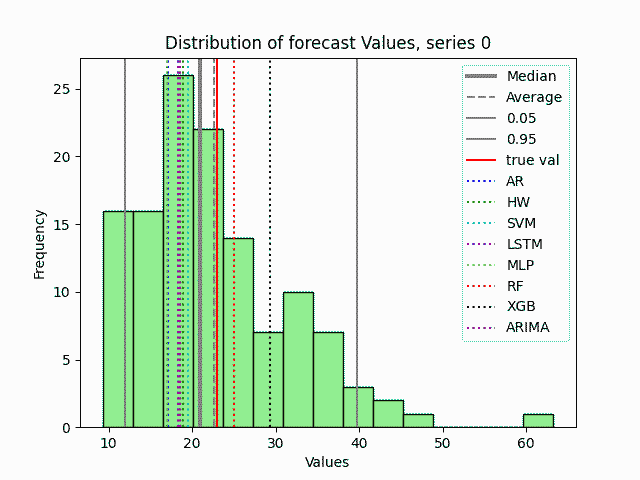
\includegraphics[width=\linewidth]{figs/distr_75_0.png}
		\label{fig:dista}%
		\vspace{0.45em}
		\textit{(a) 75 bootset, customer 0}
	\end{minipage}
	\hfill
	\begin{minipage}{0.48\textwidth}
		\centering
		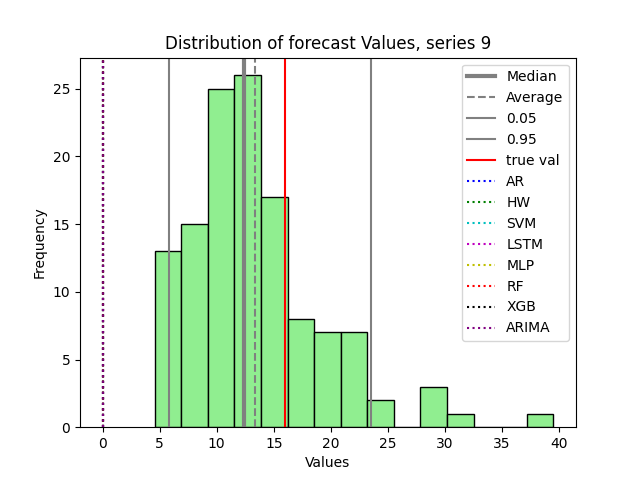
\includegraphics[width=\linewidth]{figs/distr_125_9.png}
		\label{fig:distb}%
		\vspace{0.45em}
		\textit{(b) 125 boostset, customer 9}
	\end{minipage}
    }
    { }
\end{figure}

The forecasts were compared using three cost functions: mean absolute error (MAE), mean squared error (MSE) and bias. Appendix \ref{app:errcost} reports the error values, rather than the rank-based values, for all boostset sizes. 

%Table \ref{table:YWARranks} presents the results of comparing the forecasts obtained using standard algorithms with those obtained using boosting. The boosted series were computed using an AR(5) model based on Yule-Walker equations. The forecasts of these series were obtained using a simple autoregressive model. The boosted sets consisted of 75, 125, and 175 series, which are labelled $YW\_AR\_75$ (standing for Yule-Walker, AutoRegressive, 75 series bootstrap set), $YW\_AR\_125$, and $YW\_AR\_175$, respectively.

%The columns show the average ranking of each cost function (MAE, MSE or bias) for each boostset size, while on the rows we report:
%	 $fcast\_avg$: boost forecast obtained as the average of the corresponding ranks;
%	 $fcast\_50$: boost forecast obtained as the median of the corresponding ranks;
%	 $yar$: non-boost forecast obtained by an AR model;
%	 $yarima$: non-boost forecast obtained by an ARIMA model;
%	 $yhw$: non-boost forecast obtained by a Holt and Winters model;
%	 $ymlp$: non-boost forecast obtained by a multilayer perceptron model;
%	 $ysvm$: non-boost forecast obtained by a SVM model;
%	 $ylstm$: non-boost forecast obtained by a LSTM model;
%	 $yrf$: non-boost forecast obtained by a random forest model;
%	 $yxgb$: non-boost forecast obtained by a XGboost model.
%The table shows that boosting is consistently the most reliable method for minimizing forecast errors, even when forecasts are %obtained from a model as simple as AR($p$), while ARIMA produces the least bias.
%
%\begingroup
%\renewcommand{\arraystretch}{0.40}
%\setlength{\extrarowheight}{-2pt}
%\begin{table}
%	\centering
%	\begin{tabularx}{\textwidth}{l|CCC|CCC|CCC}
%		& \multicolumn{3}{|c|}{YW\_AR\_75} &  \multicolumn{3}{|c|}{YW\_AR\_125}  &  \multicolumn{3}{|c}{YW\_AR\_175} \\
%		& MAE & MSE & bias & MAE & MSE & bias & MAE & MSE & bias \\
%		\hline
%		fcast\_avg& 2.67 & 2.67 & 0.08 & 2.58 & 2.58 & 0.05 & 3.83 & 3.83 & 0.04 \\
%		fcast\_50 & 3.04 & 3.04 & 0.06 & 3.19 & 3.19 & 0.04 & 2.50 & 2.50 & 0.03 \\
%		yhw       & 5.42 & 5.42 & 0.08 & 6.06 & 6.06 & 0.04 & 5.88 & 5.88 & 0.03 \\
%		yarima    & 5.73 & 5.73 & 0.05 & 6.04 & 6.04 & 0.03 & 6.08 & 6.08 & 0.02 \\
%		ysvm      & 5.88 & 5.88 & 0.08 & 5.50 & 5.50 & 0.05 & 5.50 & 5.50 & 0.03 \\
%		ylstm     & 6.02 & 6.02 & 0.06 & 5.52 & 5.52 & 0.04 & 6.27 & 6.27 & 0.02 \\
%		yar       & 6.06 & 6.06 & 0.04 & 6.54 & 6.54 & 0.02 & 6.79 & 6.79 & 0.02 \\
%		ymlp      & 6.38 & 6.38 & 0.05 & 5.98 & 5.98 & 0.03 & 6.17 & 6.17 & 0.02 \\
%		yrf       & 6.46 & 6.46 & 0.11 & 6.31 & 6.31 & 0.06 & 5.48 & 5.48 & 0.04 \\
%		yxgb      & 7.33 & 7.33 & 0.12 & 7.29 & 7.29 & 0.07 & 6.50 & 6.50 & 0.05 \\
%		\hline
%	\end{tabularx}
%	\caption{Average rankings for different boostset size.}
%	\label{table:YWARranks}
%\end{table}
%\endgroup

The relative merits of the different forecasting approaches are highlighted by critical difference diagrams based on the non-parametric Friedman test followed by a post-hoc Nemenyi test. These diagrams allow for a visual comparison of performance ranks and indicate whether the differences between classifiers are statistically significant \citep{D06}. In our case, the graphs were generated using the SciKit version \citep{SciKitCD} and plot the average rank across all series for each algorithm along the x-axis. Horizontal bars connect those that could not be considered statistically different.
We report here ranking results, where ranks are computed on the corresponding forecasts for each series according to the quality of the considered function to emphasize how the algorithms perform relative to each other. Then, the rank of each function is averaged over all series.  

Figures \ref{fig:ywar75} and \ref{fig:ywar175} show a comparison of the ranks on MAE for the 75 series boostset and on MSE for the 175 series boostset. Bootstrap point forecasts were obtained using the mean (fcast\_avg) or median (fcast\_50) of replicate forecasts.
In both cases, as with all those tested (see Appendix \ref{app:errcost}), the accuracy of the boost forecasts is significantly higher than that obtained with alternative models. The results are consistent across bootstrap sizes for MAE and MSE (Appendix \ref{app:errcost}). Bias rankings differ, although the absolute reported bias remains below 1\% of the empirical mean for all methods.

\begin{figure*}
	\centering
	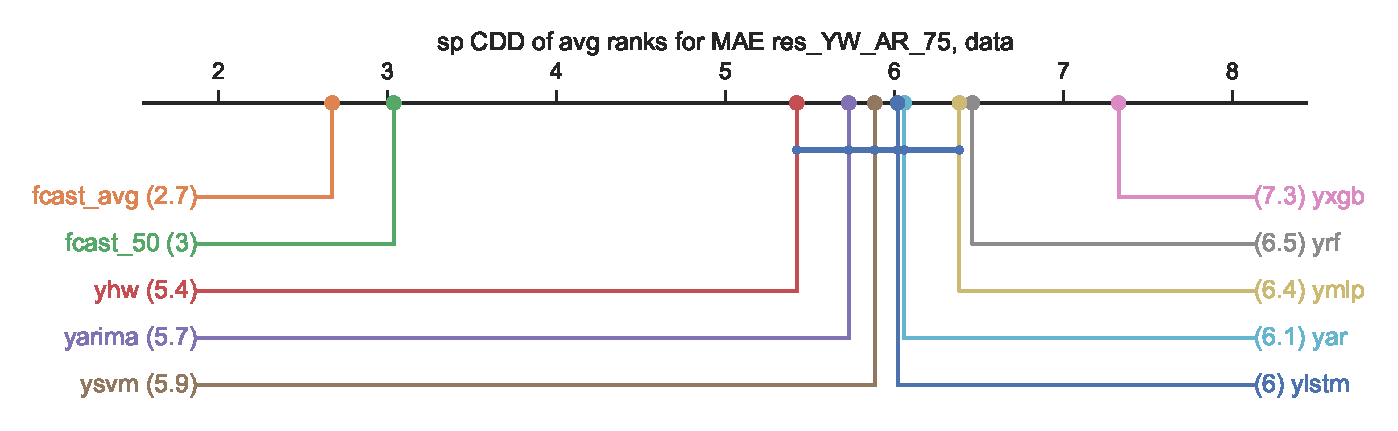
\includegraphics[width=0.75\linewidth]{figs/sp_MAE_res_YW_AR_75.eps}%
	\caption{Average ranks for MAE on instance res\_YW\_AR\_75 (Yule-Walker, AR, 75 scenarios)}
	\label{fig:ywar75}
\end{figure*}

\begin{figure*}
	\centering
	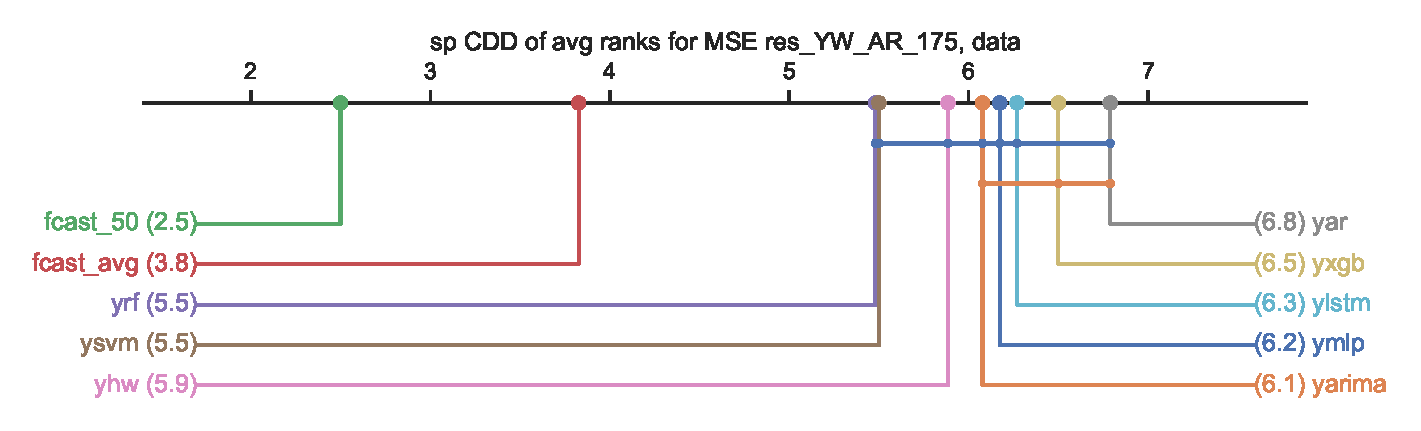
\includegraphics[width=0.75\linewidth]{figs/sp_MSE_res_YW_AR_175.eps}%
	\caption{Average ranks for MSE on instance res\_YW\_AR\_175 (Yule-Walker, AR, 175 scenarios)}
	\label{fig:ywar175}
\end{figure*}

%Our relatively short time series require a forecasting approach that can handle both limited data and non-stationarity.  Although sophisticated machine learning models such as recurrent neural networks (RNNs) and gradient boosting machines (GBMs) have become more popular in recent years, they can perform less well when there is limited data available, particularly when the data has non-stationary properties. This can lead to overfitting. The autoregressive (AR) model combined with MEB offers a powerful and promising alternative.  This technique performed excellently in the context of this study, consistently outperforming more complex machine learning models. It offers an approach based on robust statistical principles that mitigates the risk of overfitting inherent in many AI approaches. Moreover, the AR model combined with the bootstrap methodology provides reliable forecasts ideally suited to integration into the subsequent optimization module.  

The tested AR–bootstrap structure combines competitive predictive accuracy with an interpretable base forecasting model.

% ==================================================================================================================
\subsection{Prescriptive module tests}  \label{Subsec:prescrtest}

The validation of the BESO framework was obtained comparing 4 different appraoches to the solution of the test case instnce:
\begin{description}
\item[SAP] the baseline deterministic code using bagged bootstrap forecasts;
\item[BESO-SAA] the SAA version of BESO;
\item [ETS] an alternative SAA deterministic equivalent based on ETS forecasts.
\item[BESO-DRO] the DRO version of BESO;
\item [WEK] a Wasserstein-based code structured following \cite{EK18};
\end{description}

{\it The ETS realiztion} was obtained using a parametric method which assumed a Gaussian distribution of forecasts from the request datasets. This comparison was conducted using scenarios derived from a Gaussian distribution based on the confidence intervals of the forecasts provided by an Holt-Winters ETS model \citep{HKOS08}.

For WEK, for each historical rolling forecast origin $t$ and each store $j$, we compute the three-step-ahead empirical forecast error $ e_{t,j}^{(3)} = y_{t+3,j}-\hat y_{t+3|t,j} $. For the validation, we use the same AR predictor adopted in BESO, but without bootstrap resampling, which is an integral part of our proposal. We do not center the ambiguity set directly on the 45 raw monthly observations, since the series are short and nonstationary, and demand at the target seasonal period cannot be regarded as exchangeable with that of arbitrary historical months.
Using a minimum training length of 24 observations for the AR recursions yields 18 admissible forecast origins. The errors associated with each origin are retained jointly across stores and combined with the current three-step-ahead forecasts, thereby generating $N=18$ predictive demand scenarios $\rho^s$, $s\in S$. These scenarios provide a non-bootstrap empirical representation of predictive uncertainty and define the finite support of the Wasserstein benchmark.

Given these input data, we ran experiments first to assess the effectiveness of each model on the use case data, then we study the impact of the variation of the remaining sets of parameters of the formulation, i.e., cardinality of the boostsets, number of splittable stores, and assumptions on inventory costs. These test reports on the sensitivity of the solution to variations in the instance coefficients. Appendix B of the Electronic Companion provides an initial study of the fitness landscape for the split-assignment problem, using a set of artificial benchmark instances.

All reported tests were run on the same machine as in subsection \ref{Subsec:predtest}, all control paramaters were identified by the Optuna package \citep{optuna19}.

\subsubsection*{Test case solution}

You could report something like cost, unmet demand, leased capacity, and out-of-sample feasibility for all three. 


Table \ref{table:compETS} presents a comparison of solutions in the first two columns when no rental cost was added for the use of leased floor space and in the last two columns when the rental cost was included in the objective function. As expected, given that the constraints were less restrictive, the ETS solution is less expensive in both cases. However, in both cases, the solution was infeasible as it did not provide all the goods requested by one of the retailers. This result was obtained in a single instance; therefore, it may not have happened. However, it is significant that, even in the first instance in which we tested our model, its robustness proved important in dealing with a limit case.

\begingroup
\renewcommand{\arraystretch}{1.0}
\begin{table}
	\centering
	\begin{tabular}{l|cccccc|}
		                 & ETS  & SAP   & BESO-SAA & ETS-SAA & BESO-DRO & WEK  \\
		\hline
		Assign. Cost     &19682 & 20604 & 20529.77 &19918.27 & 20535.44 & 20516.42\\
		Optimality gap\% &   0  & 0     & 0        & 0       & 0        & 0\\
		Infeasibilities  &   0  & 0     & 0        & 0       & 0        & 0\\
        num.variables    &  416 & 416   & 19708    &  19708  & 19709    & 19784\\
        num.constraints  &  316 & 316   & 19852    &  19852  & 19952    & 25477\\
        num.non zeros    & 1040 & 1040  & 66508    &  66508  & 565184   & 662683\\
		t.Cpu            & 0.17 & 0.05  & 10.72    &   4.14  & 21.79    & 55.26\\
		\hline
	\end{tabular}
	\caption{Solution and model data on the use case instance and 75 boostrap set}
	\label{table:compETS}
\end{table}
\endgroup

Table \ref{table:resETS} details the proposed usage of the  DCs in the different cases. It appears that DC 2, the biggest owned one, is the overloaded one in both cases, even though by small amounts. 

\begingroup
\renewcommand{\arraystretch}{1.0}
\setlength{\tabcolsep}{3pt}
\small
\begin{table}
	\centering
	\begin{tabular}{l|ccc|ccc|ccc|ccc|ccc|ccc|}
		\multicolumn{1}{c|}{} & \multicolumn{3}{c|}{ETS} & \multicolumn{3}{c|}{SAP} & \multicolumn{3}{c|}{ETS-SAA} & \multicolumn{3}{c|}{BESO-SAA} & \multicolumn{3}{c|}{WEK} & \multicolumn{3}{c|}{BESO-DRO} \\ 
		& exp & true & ovr & exp & true & ovr & peak & true & ovr & peak & true & ovr & peak & true & ovr & peak & true & ovr \\
		\hline
		DC 0 & 119 & 115 & 0 & 120 & 111 & 0 & 120 & 118 & 0 & 120 & 111 & 0 & 120 & 111 & 0 & 120 & 111 & 0 \\
		DC 1 & 339 & 431 & 0 & 482 & 459 & 0 & 481 & 436 & 0 & 483 & 462 & 0 & 481 & 459 & 0 & 481 & 459 & 0 \\
		DC 2 & 277 & 304 & 4 & 300 & 288 & 0 & 298 & 299 & 0 & 300 & 289 & 0 & 298 & 288 & 0 & 298 & 288 & 0 \\
		DC 3 & 166 & 173 & 0 & 180 & 180 & 0 & 165 & 170 & 0 & 180 & 161 & 0 & 180 & 165 & 0 & 180 & 165 & 0 \\
		\hline
	\end{tabular}
	\caption{DC usage (expected, realized demand, realized overload per method)}
	\label{table:resETS}
\end{table}
\endgroup

Finally, we note that Table \ref{table:compETS} shows that including the rental cost makes otherwise identical instances much harder to solve. In fact, the time limit of 3600 CPU seconds was too short to reach optimality, and a duality gap was left in the proposed solutions, a substantial one in the case of the BESO instance.


Figure \ref{fig:compDistr75} shows the distributions of the forecasts of the 75 boostset obtained by BESO and by ETS. Note that the BESO distribution, given its MEB foundation, spans a wider range of values than the ETS distribution.
The wider distribution has an impact on the proposed allocation. We had empirical proof of this when we tested the BESO and ETS solutions on the validation data obtained by the end of the year.
% — i.e. when we finally received the data for which we were asked to provide a forecast.

\begin{figure*}
	\centering
	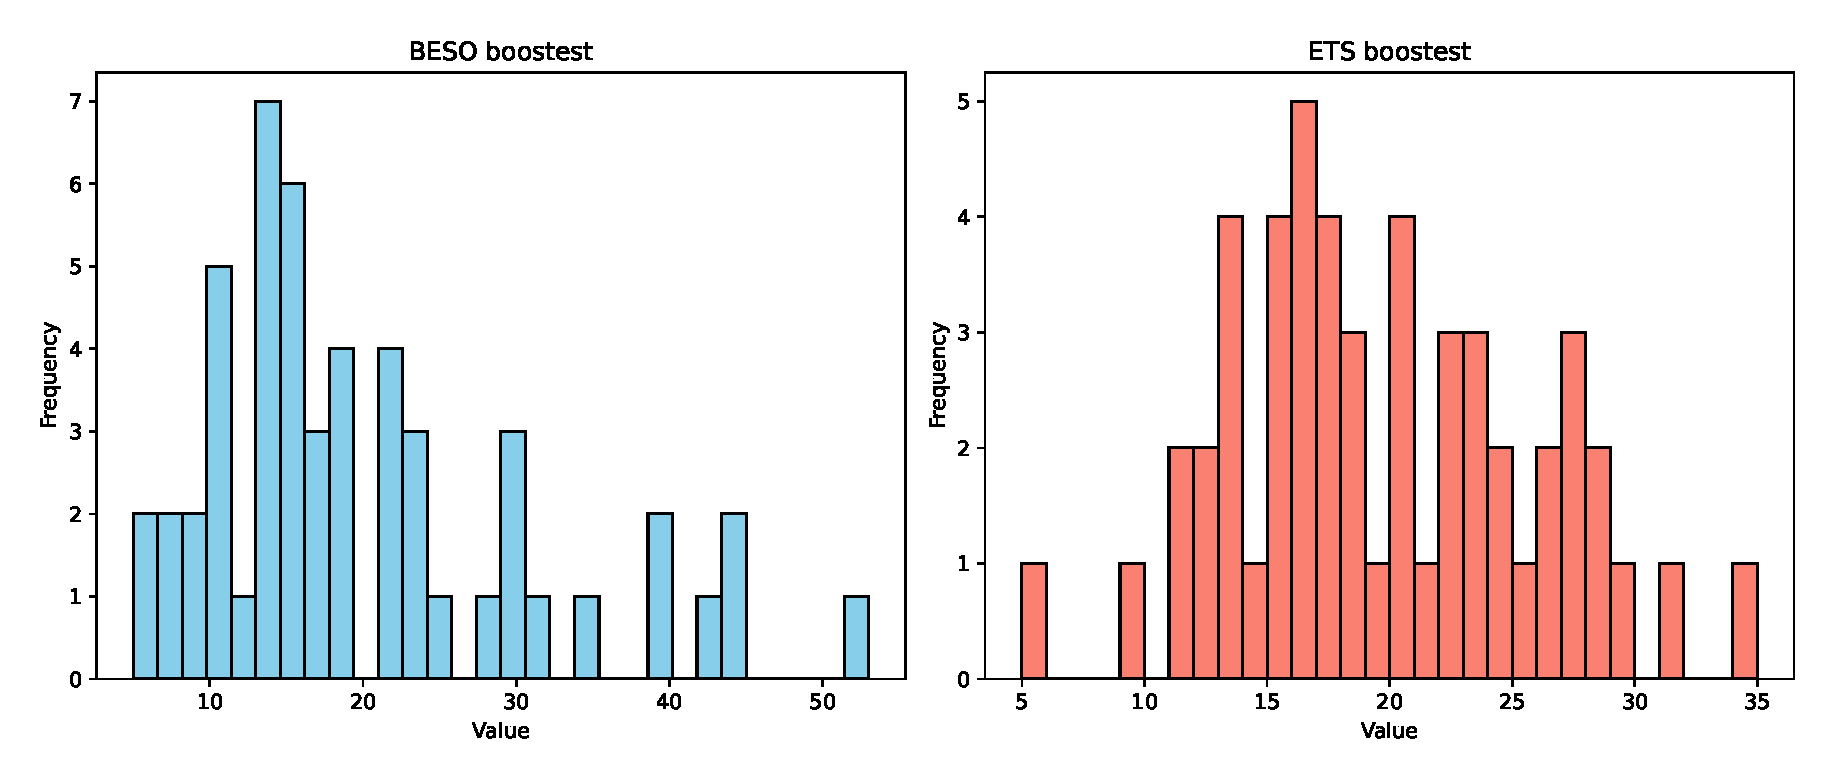
\includegraphics[width=0.75\linewidth]{figs/compDistr.eps}%
	\caption{Comparison of distributions on 75 bootstrapped series}
	\label{fig:compDistr75}
\end{figure*}

\subsubsection*{Increasing boostset size}

The size of the boostset helps to stabilize the results during forecasting, as introduced in subsection \ref{Subsec:predictive}, but it also has a deep impact on the optimization. In fact, the number of variables and constraints in the DE formulation do not depend on the size of the boostset, larger boostsets are more likely to contain unusual values or combinations thereof. This makes the constraints in equation (\ref{DErequest}) progressively harder to satisfy, which increases the cost and may render the instance infeasible.
To ascertain this, we conducted experiments using 75, 125 and 175 series boostsets, with a time limit of 600 seconds on the optimization process. Figure \ref{fig:bsize} shows a boxplot diagram depicting the distribution of the optimized cost over a number of tests equal to 1/5 of the number of series in the boostset, i.e., 15, 25, 35, respectively.

\begin{figure*}
	\centering
	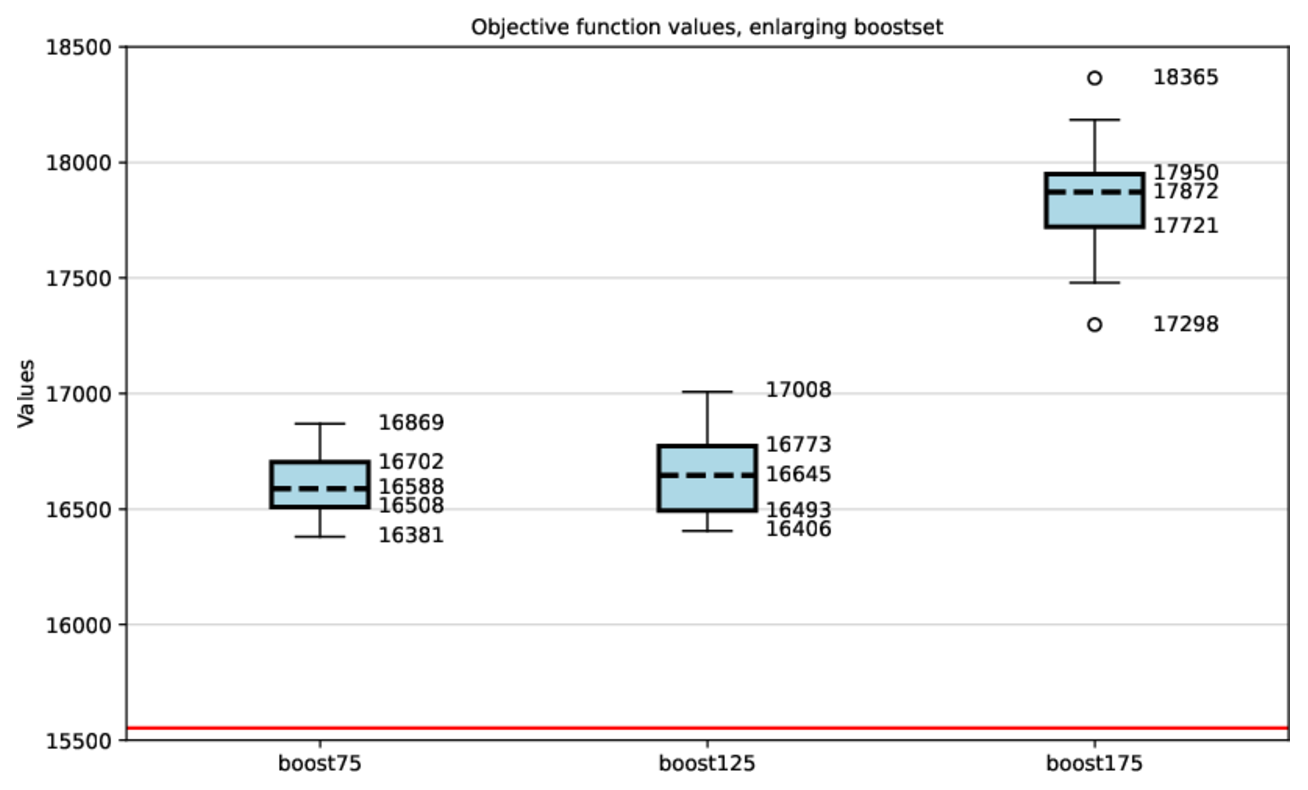
\includegraphics[width=0.7\linewidth]{figs/figb0.eps}%
	\caption{Allocation cost for increasing boostset size}
	\label{fig:bsize}
\end{figure*}

Figure \ref{fig:bsize} has a red horizontal line at the cost value for the deterministic case. Therefore, the increase in cost can be considered a quantification of the value of information about storage requests. We observe that the cost remains relatively stable for the 75 and 125 series sets, but increases significantly for the 175 boostset. This is due to the increased difficulty of the larger boostset instances, which meant that some could only be solved heuristically within the time limit. While all instances were feasible, seven out of 35 still had a gap between the lower and upper bounds after 600 seconds of CPU time. 

Finally, we note that, as expected, taking the optimal solution obtained with the coefficients imposed by the 75 series and evaluating it with the coefficients of the 125 series results in a more costly solution than that computed with the 125 series coefficients. More interestingly, however, this solution is not feasible with the 175 series coefficients.


For your 125 trajectories, for BESO I would initially use

$$
L=25,\qquad K=50.
$$

Thus, generate 50 empirical distributions, each based on 25 draws from the 125 trajectories. Because sampling is with replacement, you are not restricted to five disjoint groups.

I would then perform sensitivity tests with

$$
L\in\{10,25,50\}.
$$

Their interpretation is:

* \(L=10\): dispersed empirical distributions and relatively strong robustness;
* \(L=25\): reasonable intermediate specification;
* \(L=50\): distributions closer to the cost-aware reference distribution and milder robustness.

I would use \(L=5\) only as a deliberately conservative stress test. With five atoms, the worst of many group averages can be dominated by accidental composition.

The number \(K\) controls how thoroughly you explore the space of plausible distributions. Values around \(25\)–\(50\) should be adequate for an initial implementation; increasing \(K\) makes it more likely that an adverse empirical distribution is included.

Computationally, this need not create \(K L\) separate recourse models. You retain only the 125 original scenario-specific recourse blocks \(Q(x,\rho^s)\); the \(K\) distributions merely give you \(K\) different vectors of coefficients \(w_{ks}\) and hence \(K\) epigraph constraints.


\subsubsection*{Increasing number of splittable stores}

A defining feature of the problem we face is the possibility of accepting split service for some stores. This is unusual for allocation problems and results from the requirement to perform specific what-if analyses on the results. The number of stores allowed to split, and which ones they are, is given in input. In the actual case, the service to a store, if splittable, could be split between at most two DCs, and the quantities delivered had to be integers, as specified in all formulations.

The stores to be split are chosen from the most requesting stores. We ran a series of tests based on 75 series boostsets, allowing the 0, 4, 8, and 12 most requesting stores to be split. Figure \ref{fig:bmult} shows the corresponding boxplots.

\begin{figure*}
	\centering
	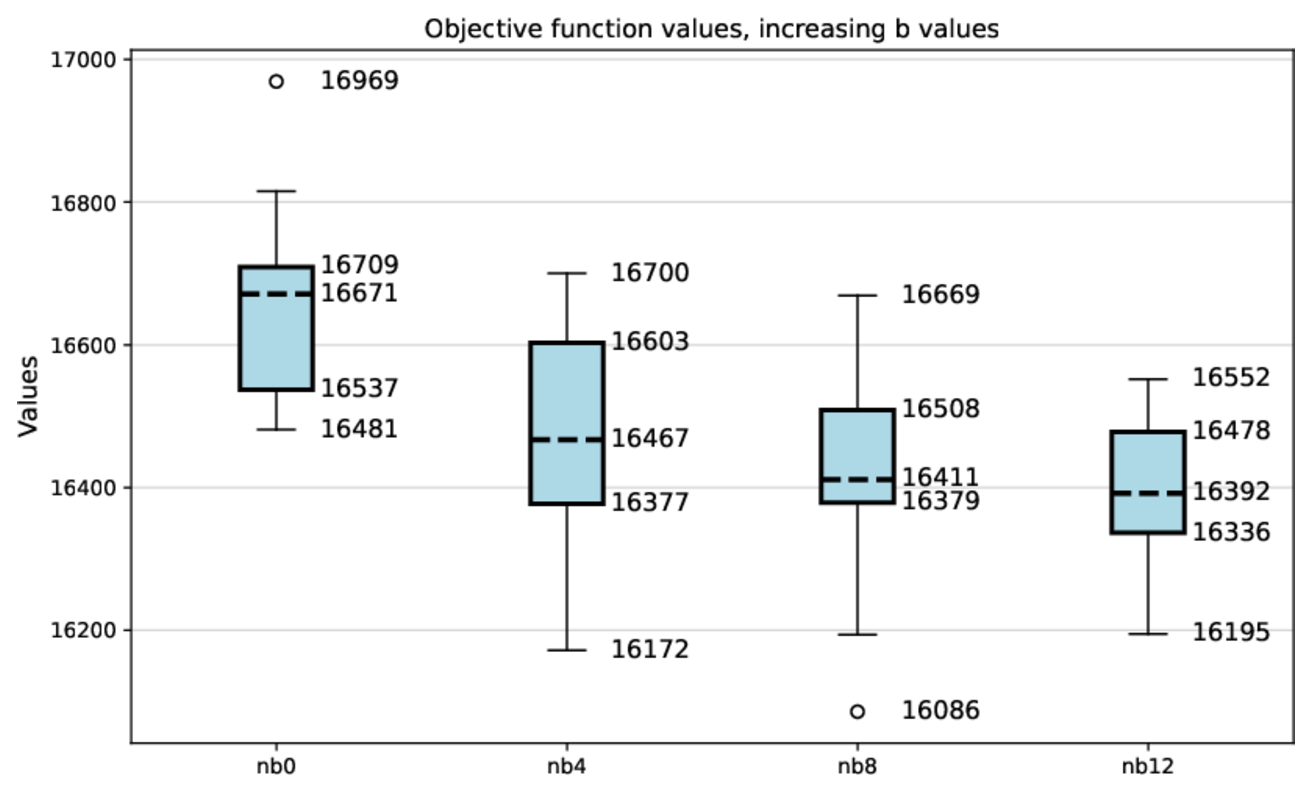
\includegraphics[width=0.65\linewidth]{figs/figbmult.eps}%
	\caption{Allocation cost for increasing number of splittable stores}
	\label{fig:bmult}
\end{figure*}

Allowing a service to be split for a store is a partial relaxation of the corresponding assignment constraint, so the expected optimal cost is lower. This can indeed be seen in figure \ref{fig:bmult}, where the more stores that are permitted to split, the lower all distribution moments become. However, the marginal decrease becomes smaller as the number of stores who can split increases, since splitting a small store may result in only a small contribution, if any.

\subsubsection*{Impact of different inventory cost assumptions}

A further set of tests was conducted to determine the impact of inventory costs $h_i$, $i \in I$ on the search process. Recall that in the original case study, one of the objectives was to determine how much space should be rented in the only DC not owned by the company, where storage space needs to be leased. The data of the case study proposed in \citet{MZ23} did not report storage costs. Here, we consider storage costs that are inversely proportional to the average distance of the DC from the stores. We consider three settings, one with no storage costs, one where only the most distant DC incurs costs, and one where all DCs need to lease space. Costs are proportional to the quantities stored and are therefore influenced by the allocation policy.

All the tests were performed using the 75-series boost set. The focus of the analysis is not on the increase in optimal costs, since an increase in the costs of the decision variables clearly leads to an increase in the total costs. Rather, the focus is on the variation in the complexity of the search, as reflected in the CPU time required to reach the final result, and on the optimality or feasibility of the solutions. To evaluate the effectiveness of increasingly lengthy searches, we present results after 600, 1200, and 3600 seconds of CPU time.
The results are summarized in the table \ref{table:qcost}. All results are based on 15 repetitions, and the columns show:
	 $n$: number of stores (stores);
	 $m$: number of DCs;
	 $n_{boost}$: number of series in the boostset;
	 $n_q$: number of DCs incurring leasing costs;
	 $n_{inf}$: number of infeasible solutions at the end of the search;
	 {\it GAP lin}: average gap between the linear bound and the best solution at the end of the search;
	 {\it GAP fin}: average gap between the best lower bound and the best solution at the end of the search;
	 {\it t.CPU}: average CPU time (in sec) of the search process.
\begingroup
\renewcommand{\arraystretch}{0.50}
\begin{table}
	\centering
	\renewcommand{\arraystretch}{1.0}
	\begin{tabularx}{0.8\textwidth}{CCCC|CCCC}
		$n$ & $m$ & $n_{boost}$ & $n_q$ & $n_{inf}$ & GAP~lin & GAP~fin & t.CPU \\
		\hline
		52 & 4 & 75        & 0 & 0    & 0.01    & 0.00    &  333.95 \\
		\hline
		52 & 4 & 75        & 1 & 1    & 0.18    & 0.17    &   600  \\
		52 & 4 & 75        & 1 & 0    & 0.15    & 0.14    &  1200 \\
		52 & 4 & 75        & 1 & 0    & 0.14    & 0.13    &  3600 \\
		\hline
		52 & 4 & 75        & 2 & 0    & 0.04    & 0.04    &   600 \\
		52 & 4 & 75        & 2 & 0    & 0.01    & 0.03    &   1200 \\
		52 & 4 & 75        & 2 & 0    & 0.01    & 0.03    &   3600 \\
		\hline
		52 & 4 & 75        & 3 & 0    & 0.01    & 0.00    &  211.03 \\
		\hline
		52 & 4 & 75        & 4 & 0    & 0.01    & 0.00    &  13.00 \\
		\hline
	\end{tabularx}
	\caption{Gap and CPU time for increasing number of leased DCs.}
	\label{table:qcost}
\end{table}
\endgroup

Table \ref{table:qcost} illustrates an interesting feature of the fitness landscape of this split-cost allocation problem: the complexity of the search is not monotonic with respect to the number of leased DCs. In fact, CPLEX was able to solve all instances to optimality for 0, 3 and 4 leased DCs. However, for 1 or 2 leased DCs, it was never able to prove the optimality of the best solution found within the time limit of 3600 seconds. Furthermore, instances with one leased DC are more challenging than those with two, as demonstrated by the gap between the lower and upper bounds, both between the linear relaxation bound and the best solution found and between the best final lower bound and the best solution. This feature is discussed further in Appendix B of the Electronic Companion.

As a final note, we point out that the objective function was structured to lexicographically first strive for feasibility and then optimize within the feasible domain. In fact, all instances have always resulted in feasible solutions. Reducing the cost coefficient of the request slack variables allows us to explore the trade-off between solution cost and the probability of reaching an infeasible solution. However, we did not explore this further.

\section{Conclusions and future directions} \label{Sec:conclusions}

This paper introduces Bootstrap Enhanced Scenario Optimization (BESO), a framework for deriving predictive prescriptions from  relevant data series. It integrates statistically grounded forecasting with scenario-based optimization by generating future scenarios via bootstrapped autoregressive time series, while incorporating feedback from the optimization stage. A two-echelon logistics case study illustrates how BESO forecasts retailer demand and supports DC allocation, enabling decisions on inventory, capacity, and assignment that reflect both cost structures and uncertainty.

A central contribution of BESO is providing a credible alternative to traditional Distributionally Robust Optimization (DRO). Standard DRO methods rely on predefined ambiguity sets (e.g., moment bounds, Wasserstein metrics, $\phi$-divergences), which may fail to capture complex empirical features such as nonstationarity or heavy tails. BESO instead constructs empirical scenario distributions via Maximum Entropy Bootstrap (MEB), avoiding explicit ambiguity sets. It also allows an objective-aware extension, where optimization-related costs inform the resampling process, producing scenarios aligned with decision quality. The bootstrap size further acts as a transparent control over robustness, replacing exogenous parametric design.

Experiments on real and synthetic data show that BESO yields robust, interpretable prescriptions and adapts well to varying uncertainty structures, achieving performance comparable to classical scenario generation and DRO approaches. Overall, integrating forecasting and optimization within a unified empirical loop enhances both stability and operational effectiveness.

Future research may further explore bootstrap-based ambiguity representations, positioning BESO as a data-driven DRO alternative. Extensions could include hybrid schemes incorporating prior knowledge or Bayesian elements, as well as broader applicability to settings where reliable forecasting models are not available.

add one sentence noting the natural extension to aleatoric noise (augmenting each trajectory with resampled residuals),

% References 
\bibliographystyle{informs2014} % 
\bibliography{GDObiblio} % if more than one, comma separated

% Appendix
% --- Start Appendices Here ---
\appendix
\vspace*{-10pt}
\section{Appendix A: Cost function values} \label{app:errcost}

This section reports the absolute values of the various cost functions, which were calculated using the forecast errors obtained by averaging the corresponding errors for each of the 52 test case series described in the paper.

\begin{table}[h]
	\centering
	\renewcommand{\arraystretch}{1.0}
	\begin{tabular}{ccccccc}
		model & bias & MAPE & ME & MAE & MPE & RMSE \\
		\hline
		fcast\_50   &-0.27 & 0.09 &-1.02 & 1.63 &-0.05 &  2.12 \\
		fcast\_avg  & 0.02 & 0.07 & 0.07 & 1.25 & 0.01 &  1.68 \\
		yar         & 0.36 & 0.34 & 1.36 & 5.86 & 0.07 &  9.75 \\
		yhw         & 0.63 & 0.34 & 2.41 & 5.99 & 0.13 & 10.59 \\
		ysvm        & 0.69 & 0.36 & 2.66 & 6.20 & 0.14 & 10.99 \\
		ylstm       & 0.56 & 0.35 & 2.13 & 6.01 & 0.11 & 10.41 \\
		ymlp        & 0.47 & 0.36 & 1.79 & 6.26 & 0.09 & 10.60 \\
		yrf         & 1.50 & 0.44 & 5.73 & 7.79 & 0.31 & 13.54 \\
		yxgb        & 2.28 & 0.58 & 8.74 &10.12 & 0.49 & 17.05 \\
		yarima      & 0.44 & 0.34 & 1.67 & 5.80 & 0.09 &  9.77 \\
		\hline
	\end{tabular}
	\caption{Error costs for the 75 series boostset.}
	\label{table:app75}
\end{table}

\begin{table}[h]
	\centering
	\renewcommand{\arraystretch}{1.0}
	\begin{tabular}{ccccccc}
		model & bias & MAPE & ME & MAE & MPE & RMSE \\
		\hline
		fcast\_50   & -0.56 & 0.09 & -1.08 & 1.59 & -0.06 & 2.25  \\
		fcast\_avg  &  0.02 & 0.07 &  0.05 & 1.18 &  0.01 & 1.65  \\
		yar         & -0.59 & 0.25 & -1.13 & 4.36 & -0.07 & 6.31  \\
		yhw         & -0.13 & 0.24 & -0.26 & 4.33 & -0.02 & 6.39  \\
		ysvm        & -0.06 & 0.24 & -0.11 & 4.18 & -0.01 & 6.39  \\
		ylstm       & -0.30 & 0.24 & -0.58 & 4.15 & -0.04 & 6.34  \\
		ymlp        & -0.47 & 0.24 & -0.90 & 4.22 & -0.05 & 5.99  \\
		yrf         &  1.27 & 0.28 &  2.44 & 5.01 &  0.14 & 7.48  \\
		yxgb        &  2.52 & 0.38 &  4.85 & 6.52 &  0.28 & 9.46  \\
		yarima      & -0.40 & 0.25 & -0.76 & 4.44 & -0.05 & 6.83  \\
		\hline
	\end{tabular}
	\caption{Error costs for the 125 series boostset.}
	\label{table:app125}
\end{table}

\begin{table}[h]
	\centering
	\renewcommand{\arraystretch}{1.0}
	\begin{tabular}{ccccccc}
		model & bias & MAPE & ME & MAE & MPE & RMSE \\
		\hline
		fcast\_50  & -0.04 & 0.07 & -0.07 & 1.22 & 0     & 1.51 \\
		fcast\_avg & 0.99  & 0.12 & 1.90  & 2.04 & 0.12  & 2.76 \\
		yar        & -0.22 & 0.35 & -0.42 & 5.84 & -0.03 & 7.64 \\
		yhw        & 0.25  & 0.34 & 0.48  & 5.75 & 0.02  & 7.90 \\
		ysvm       & 0.30  & 0.33 & 0.58  & 5.66 & 0.03  & 7.76 \\
		ylstm      & 0.10  & 0.34 & 0.20  & 5.76 & 0     & 7.74 \\
		ymlp       & -0.19 & 0.34 & -0.36 & 5.69 & -0.02 & 7.57 \\
		yrf        & 1.72  & 0.37 & 3.31  & 6.39 & 0.18  & 9.66 \\
		yxgb       & 3.01  & 0.46 & 5.78  & 7.96 & 0.33  & 11.83\\
		yarima     & -0.04 & 0.34 & -0.08 & 5.69 & -0.01 & 7.63 \\
		\hline
	\end{tabular}
	\caption{Error costs for the 175 series boostset.}
	\label{table:app175}
\end{table}

The functions reported in the columns are: bias, Means Absolute Percentage Error (MAPE), Mean Error (ME), Mean Absolute Error (MAE), Mean Percentage Error (MPE) and Root Mean Square Error (RMSE). Table \ref{table:app75} gives the cost values for the case of a boost set composed of 75 series, table \ref{table:app125} for the 125 series and table \ref{table:app175} for the 175 series sets.

All tables show significantly consistent results across all boost set sizes.

\section{Appendix B: Extended deterministic benchmark set} \label{app:artificial}

All analyses reported in sections \ref{Subsec:predictive} and \ref{Subsec:prescriptive} refer to the case study at the heart of this paper, but the interest of the method is not limited to this particular case study as it can be effective on any instance of this 2-echelon supply chain problem. To test the generality of the results, we generated a benchmark set with varying dimensions and coefficients. The study was conducted only with respect to the deterministic setting, and is therefore significant for assessing the computational complexity of the split-allocation problem as a deterministic combinatorial optimization problem.

We generated 5 instances for each configuration of number of stores ($n$), number of DCs ($m$), and number of splittable stores. The travel costs were obtained by randomly selecting $m$ rows and $n$ columns from a large distance matrix, whose values were computed as the actual road distances between points located in the same area as the test case. DC inventory costs were inversely proportional to the average travel cost from the DC to the stores and store requests were inversely proportional to the average travel cost from the store to the DCs. Note that the distance matrix is asymmetric, as it was computed within a city area. The number $n_b$ of splittable stores was progressively increased as the number $n_q$ of DCs with nonzero inventory costs. Specifically, the range of the defining parameters were: $n$: \{50, 52, 100, 200, 300\}, $m$: \{4, 5, 10, 25, 50\}, $n_b$: \{0, 4, 5, 10, 25, 50\}, $n_q$: \{0, 1, 2, 3, 4, 5\}.

Not all combinations of values were generated, the larger values were used only for instances with higher number of stores. In particular, the values 4 and 52 were only used to generate instances with the same dimensionality as the case study, in order to check the generality of the results obtained. The first instance of this set was kept to be the case study one.

The computational results in the case of no costly DC, reported as averages over the 5 generated instances, are summarized in table \ref{table:extset}, whose columns show:
\begin{itemize}
	\item $n$, $m$: number of stores and number of DCs;
	\item $n_b$: maximum number of splittable stores;
	\item $ncols$, $nrows$: number of columns and number of rows in formulation FD;
	\item $gaplb$: average percentage gap between the linear relaxation lower bound and the cost of the best solution found;
	\item $gapfinal$: average percentage gap between the best lower bound at the end of the search (smallest cost of an unexpanded node) and the cost of the best solution found;
	\item $ninf$: number of instances for which no feasible solution was found;
	\item $nopt$: number of instances solved to proven optimality;
	\item $tcpu$: average CPU time for solving the instance, time to optimality or 3600 if optimality could not be proven;
\end{itemize}

The table shows two trends. One, with respect to instance size, shows an expected increase in complexity. While instances the size of our test case are easily solved to optimality by modern solvers, increasing the size, as defined by the number of variables and the number of constraints, quickly leads to instances that could not be solved to optimality within the 3600-second time limit. 
The number of splittable stores has an important effect on the complexity of the instance. Instances of the same absolute size, but with more splittable stores, usually have a looser linear relaxation (LP) bound and have more difficulty reaching optimality, as can be seen by the decreasing number of instances out of the 5 from each group that could be solved to optimality.

\begin{table}
	\centering
	\renewcommand{\arraystretch}{1}
	\begin{tabular}{cccccccccc}
		$n$ & $m$ & $n_b$ & $ncols$ & $nrows$ & $gaplb$ & $gapfinal$ & $ninf$ & $nopt$ & $tcpu$\\
		\hline
		52 &  4 &  0 &   416 &   316 & 0.21 & 0.01 & 0 & 5 &    0  \\
		\hline
		50 &  5 &  0 &   500 &   355 & 0.39 & 0.00 & 0 & 5 &    3  \\
		50 &  5 &  5 &   500 &   355 & 0.40 & 0.00 & 0 & 5 &    4  \\
		50 & 10 &  0 &  1000 &   610 & 1.32 & 0.00 & 0 & 5 &  383  \\
		50 & 10 &  5 &  1000 &   610 & 1.34 & 0.00 & 0 & 5 &  378  \\
		50 & 10 & 10 &  1000 &   610 & 1.35 & 0.13 & 0 & 4 & 1150  \\
		\hline
		100 & 10 &  0 &  1000 &  1210 & 0.50 & 0.12 & 0 & 2 & 1920  \\
		100 & 10 &  5 &  1000 &  1210 & 0.54 & 0.05 & 0 & 3 & 1514  \\
		100 & 10 & 10 &  1000 &  1210 & 0.57 & 0.09 & 0 & 3 & 2063  \\
		100 & 50 &  0 & 10000 &  5250 & 5.23 & 3.06 & 0 & 0 & 3600  \\
		100 & 50 &  5 & 10000 &  5250 & 4.77 & 2.70 & 0 & 0 & 3600  \\
		100 & 50 & 10 & 10000 &  5250 & 4.55 & 2.42 & 0 & 0 & 3600  \\
		100 & 50 & 25 & 10000 &  5250 & 4.52 & 2.61 & 0 & 0 & 3600  \\
		\hline
		200 & 10 &  0 &  4000 &  2410 & 0.17 & 0.05 & 0 & 2 & 2369  \\
		200 & 10 &  5 &  4000 &  2410 & 0.17 & 0.09 & 0 & 1 & 2893  \\
		200 & 10 & 10 &  4000 &  2410 & 0.18 & 1.01 & 0 & 0 & 3600  \\
		200 & 50 &  0 & 20000 & 10450 & 1.66 & 1.26 & 0 & 0 & 3600  \\
		200 & 50 & 10 & 20000 & 10450 & 1.68 & 1.29 & 0 & 0 & 3600  \\
		200 & 50 & 25 & 20000 & 10450 & 1.71 & 1.37 & 0 & 0 & 3600  \\
		\hline
		300 & 10 &  0 &  6000 &  3610 & 0.09 & 0.03 & 0 & 3 & 1798 \\
		300 & 10 &  5 &  6000 &  3610 & 0.09 & 0.07 & 0 & 0 & 3600 \\
		300 & 10 & 10 &  6000 &  3610 & 1.02 & 0.47 & 0 & 0 & 3600 \\
		300 & 50 &  0 & 30000 & 15650 & 0.94 & 0.73 & 0 & 0 & 3600  \\
		300 & 50 & 10 & 30000 & 15650 & 0.93 & 0.76 & 0 & 0 & 3600  \\
		300 & 50 & 25 & 30000 & 15650 & 0.96 & 0.84 & 0 & 0 & 3600  \\
		\hline
	\end{tabular}
	\caption{Extended benchmark set, deterministic case, no costly DC}
	\label{table:extset}
\end{table}

Note that the optimality gap of the LP bound is usually small, except for the $n$=100 and $m$=50 instances, but the search still struggles to close this gap. Interestingly, the LP bound gets tighter as $n$ increases, but this does not make the search any easier.
The least-cost solution when optimality was not proven was usually found within the first 600 seconds of CPU time. However, we note that designing efficient heuristics for this problem is beyond the scope of this research. We could have tweaked the solver configuration to favor heuristic search at the expense of efficiency in proving optimality, or designed custom heuristics, but the focus here is on assessing the fitness landscape when road network costs are involved.

Table \ref{table:extsetq} reports results about tests varying the number of costly DCs, the columns show:
\begin{itemize}
	\item $n$, $m$: number of stores and number of DCs;
	\item $ncols$, $nrows$: number of columns and number of rows in formulation FD;
	\item lb0, t0: linear relaxation bound and CPU time in the case of no costly DCs;
	\item lb1, t1: linear relaxation bound and CPU time in the case of 1 costly DC;
	\item lb2, t2: linear relaxation bound and CPU time in the case of 2 costly DCs;
	\item lb3, t3: linear relaxation bound and CPU time in the case of 3 costly DCs;
	\item lb4, t4: linear relaxation bound and CPU time in the case of 4 costly DCs;
	\item lb5, t5: linear relaxation bound and CPU time in the case of 5 costly DCs;
\end{itemize}

The table reports results on two sets of instances. The top 4 rows contain aggregate results on a set of instances, 5 for each configuration, where inventory costs are directly proportional to average distances, while the bottom 4 rows have costs inversely proportional to average distances.

\begin{table}
	\addtolength{\tabcolsep}{-3pt}
	\footnotesize 
	\centering
	\renewcommand{\arraystretch}{1}
	\begin{tabular}{cccc|cc|cc|cc|cc|cc|cc}
		n & m & ncols & nrows & lb0 & t0 & lb1 & t1 & lb2 & t2 & lb3 & t3 & lb4 & t4 & lb5 & t5 \\
		\hline
		52 & 4  & 416 & 316 & 0.86 & 0.2 & 0.17 & 0.81 & 0.08 & 0.22 & 0.01 & 0.02 & 0.00 & 0.02 & - & - \\
		50 & 5  & 500 & 355 & 1.33 & 0.06 & 2.77 & 0.06 & 1.46 & 0.13 & 0.11 & 14.31 & 0.06 & 7 & 0.05 & 0.93 \\
		100 & 5 & 1000 & 705 & 0.41 & 0.24 & 0.09 & 6.39 & 0.06 & 3.2 & 0.01 & 0.06 & 0.02 & 4.8 & 0.02 & 2.71 \\
		200 & 5 & 2000 & 1405 & 0.14 & 1.43 & 0.01 & 1.79 & 0.01 & 0.25 & 0.01 & 0.17 & 0.01 & 0.11 & 0.01 & 7.84 \\
		\hline
		52 & 4  & 416 & 316 & 0.86 & 0.36 & 0.24 & 0.22 & 0.22 & 0.14 & 0.26 & 0.09 & 0.05 & 1.9 & - & - \\
		50 & 5  & 500 & 355 & 1.33 & 0.16 & 0.52 & 0.07 & 0.50 & 5.8 & 0.13 & 10.11 & 0.05 & 1.37 & 0.02 & 0.22 \\
		100 & 5 & 1000 & 705 & 0.41 & 0.33 & 0.19 & 8.58 & 0.04 & 6.14 & 0.02 & 0.41 & 0.02 & 0.58 & 0.02 & 3.78 \\
		200 & 5 & 2000 & 1405 & 0.14 & 1.55 & 0.07 & 39.07 & 0.04 & 9.44 & 0.01 & 0.12 & 0.02 & 4.48 & 0.01 & 6.66 \\
		\hline
	\end{tabular}
	\caption{Extended benchmark set, deterministic case, increasing number of costly DCs}
	\label{table:extsetq}
\end{table}

The complexity of solving instances increases non-monotonically with the number of costly DCs, for both increasing and decreasing inventory costs. While the 0-cost instances are comparatively easy to solve, the CPU time required to prove optimality increases with the addition of the first costly DCs and then decreases as more DCs are paid to store inventory. However, this is not true of the gap between the linear relaxation bound and the cost of the optimal solution, where the instances with no costly DCs always have the largest gap.
As expected, the CPU time required to prove optimality increases with the dimension, and an inverse correlation between storage cost and travel cost is more difficult to solve than the case with a positive correlation.

\section{Appendix C: DRO model properties} \label{app:proofs}
%----------------------------------------------------------------------------------------------------------------------------
% BESO-DRO: Propositions 1 and 2
% Requires amsmath, amssymb, amsthm and, e.g., in the preamble:
%   \newtheorem{proposition}{Proposition}
%   \theoremstyle{remark}\newtheorem{remark}{Remark}
%----------------------------------------------------------------------------------------------------------------------------

% ---- Recourse notation (to be aligned with the epigraph paragraph) --------------------------------------------------------
% For each scenario s, the recourse problem is written as
%   Q(x,\tau^s) = \min\{ r_s(y) : y \in Y(x,\tau^s) \},
% with recourse variables y_s (replacing q_s in the current draft, to avoid the clash with Q).

\begin{proposition}[Supremum as a maximum]\label{prop:supmax}
Suppose that, for every $x\in X$ and $s\in S$, the recourse problem $Q(x,\tau^s)=\min\bigl\{\,r_s(y)\;:\;y\in Y(x,\tau^s)\bigr\}$
is feasible and attains its minimum. Then, for every $x\in X$,
\[ \Psi_{m,d}(x)=\sup_{P\in\mathcal U_{m,d}}\mathbb E_P[c(x,\xi)]=\max_{k\in K}C_k(x), \]
and the supremum is attained at one of the generating distributions $\widehat P^{\,k}$;
\end{proposition}

\begin{proof}
All $\widehat P^{\,k}$ are supported on the finite pool $\mathcal T=\{\tau^1,\ldots,\tau^n\}$, so, by the definition of \(\mathcal U_{m,d}\) as the convex hull of the generating distributions, every \(P\in\mathcal U_{m,d}\) can be written as $P=\sum_{k\in K}\lambda_k\widehat P^{\,k}$ with weights $\lambda\in\Pi_m$. 

Since \(w_{ks}\) is the probability of scenario \(s\) under generating distribution \(\widehat P^{\,k}\), and the probability assigned by \(P\) to scenario \(\tau^s\) is \(\sum_{k\in K}\lambda_k w_{ks}\), by linearity we have
\[
\mathbb E_P[c(x,\xi)]
=\sum_{s\in S}\Bigl(\sum_{k\in K}\lambda_k w_{ks}\Bigr)c(x,\tau^s)
=\sum_{k\in K}\lambda_k C_k(x) \; \le \; \max_{k\in K}C_k(x),
\]
with equality obtained by choosing any $k^*\in\arg\max_{k\in K}C_k(x)$ and setting $\lambda_{k^*}=1$ and $\lambda_k=0$ for all $k\ne k^*$.

\noindent Since $\widehat P^{\,k^*}\in\mathcal U_{m,d}$, the supremum is a maximum attained at a generating distribution. Thus, any distribution in \(\mathcal U_{m,d}\) has an expected cost equal to a weighted average of the generating distributions’ expected costs. This average cannot exceed the largest of those costs, and choosing that generating distribution alone achieves equality.
\end{proof}

\begin{proposition}[Min-max equivalence]\label{prop:minmax}
Under the assumptions of Proposition~\ref{prop:supmax}, the BESO-DRO problem $\min_{x\in X}\Psi_{m,d}(x)$ has the same optimal value as
\begin{equation}\label{eq:dro-ext}
\begin{aligned}
\min \quad & z\\
\text{s.t.}\quad & z\;\ge\; h(x)+\sum_{s\in S}w_{ks}\,r_s(y_s), && k\in K,\\
& y_s\in Y(x,\tau^s), && s\in S,\\
& x\in X,
\end{aligned}
\end{equation}
and $x^\star$ is optimal for BESO-DRO if and only if there exist $z^\star$ and $y_s^\star$, $s\in S$, such that $(x^\star,z^\star,y^\star)$ is optimal for \eqref{eq:dro-ext}.
\end{proposition}
\begin{proof}
Fix $x\in X$ and let $Y(x)=\prod_{s\in S}Y(x,\tau^s)$. For fixed $(x,y)$ the smallest feasible $z$ equals $\max_{k\in K}\{h(x)+\sum_{s}w_{ks}r_s(y_s)\}$, so the optimal value of \eqref{eq:dro-ext} with $x$ fixed is
\[
G(x)=\min_{y\in Y(x)}\ \max_{k\in K}\Bigl\{h(x)+\sum_{s\in S}w_{ks}\,r_s(y_s)\Bigr\}.
\]
For any $y\in Y(x)$ we have $r_s(y_s)\ge Q(x,\tau^s)$ for every $s$; since $w_{ks}\ge 0$, each term in the maximum is at least $C_k(x)$, hence $G(x)\ge\max_{k}C_k(x)$. 

Conversely, choose $y_s^\star(x)\in\arg\min\{r_s(y):y\in Y(x,\tau^s)\}$ for each $s$. This choice does not depend on $k$, and with it every term equals $C_k(x)$ simultaneously, so $G(x)\le\max_k C_k(x)$. Therefore $G(x)=\max_k C_k(x)=\Psi_{m,d}(x)$ by Proposition~\ref{prop:supmax} and minimizing over $x\in X$ gives equal optimal values.

Therefore, if $x^\star$ is optimal for BESO-DRO, then $(x^\star,\Psi_{m,d}(x^\star),y^\star(x^\star))$ is feasible for \eqref{eq:dro-ext} and attains its optimal value. Conversely, if $(x^\star,z^\star,y^\star)$ is optimal for \eqref{eq:dro-ext}, then $\Psi_{m,d}(x^\star)=G(x^\star)\le z^\star=\min_{x\in X}\Psi_{m,d}(x)$, so $x^\star$ is optimal for BESO-DRO.
\end{proof}

\begin{remark}
Problem~\eqref{eq:dro-ext} has the same recourse variables as BESO-SAA, plus one scalar $z$, and replaces the single SAA objective by $m$ epigraph constraints. If each $r_s$ is linear and each $Y(x,\tau^s)$ is polyhedral, \eqref{eq:dro-ext} is an LP or MILP of essentially the same size as BESO-SAA. 
\end{remark}

\begin{proposition}[Problem reduction]\label{prop:probred}
Let $S_0=\{s\in S: w_{ks}=0, k\in K\}$ be the set of scenarios assigned zero weight by every generating distribution, thus never drawn. Removing from \eqref{eq:dro-ext} the variables $y_s$ and the constraints $y_s\in Y(x,\tau^s)$ for $s\in S_0$ leaves the optimal value and the set of optimal first-stage decisions unchanged.
\end{proposition}

\begin{proof}
For $s\in S_0$ the variable $y_s$ has zero coefficient in every epigraph constraint; its only role is through $y_s\in Y(x,\tau^s)$, which is satisfiable for every $x\in X$ by relatively complete recourse. The reduced problem is thus the projection of \eqref{eq:dro-ext} that drops $y_s$, $s\in S_0$, and has the same feasible first-stage decisions and objective values.
\end{proof}

% ---- Probabilistic construction (needed to make the limits in d and m well defined) --------------------------
We fix the following construction in order to define the limit proporties induced by $d$ and $m$, given the scenario pool and $p^{\mathrm{OA}}$. 
Let $\{I_{k\ell}\}$, $k\in K$ and $1 \leq\ell\leq d$, be a set of independent random indices with $p(I_{k\ell}=s)=p^{\mathrm{OA}}_s$, $s\in S$. A resample $k$ of size $d$ consist of $I_{k1},\ldots,I_{kd}$, so that the weight \(w^{(d)}_{ks}\) is the relative frequency of scenario \(s\) in the \(k\)-th resample of size \(d\), 
$\widehat P^{\,k}=\sum_{s\in S}w^{(d)}_{ks}\,\delta_{\tau^s}$ and $\mathcal U_{m,d}=\operatorname{conv}\{\widehat P^{\,1},\ldots,\widehat P^{\,m}\}$.

The number of resamples increases with $m$ and the number of draws within each resample increases with $d$.
The BESO-SAA objective is $\Phi(x)=\sum_{s\in S}p_s^{\mathrm{OA}}c(x,\tau^s)$, $z_{\mathrm{SAA}}=\min_{x\in X}\Phi(x)$, $z_{m,d}=\min_{x\in X}\Psi_{m,d}(x)$, and $\mathcal P(\mathcal T)=\{\sum_{s\in S}\lambda_s\delta_{\tau^s}:\lambda\in\Pi_n\}$ is the set of all distributions supported on the scenario pool.

\begin{proposition}[Monotonicity in $m$]\label{prop:monoton}
For fixed \(d\), let \(\mathcal U_{m,d}\) be the convex hull of the first \(m\) distributions of a common sequence of generating distributions. Then, for every \(m\geq1\), $\mathcal U_{m,d}\subseteq\mathcal U_{m+1,d}$. Hence $\Psi_{m,d}(x)\le\Psi_{m+1,d}(x)$ for every $x\in X$, and $z_{m,d}\le z_{m+1,d}$.
\end{proposition}

\begin{proof}
The generating set of $\mathcal U_{m+1,d}$ contains that of $\mathcal U_{m,d}$, and the convex hull is monotone with respect to inclusion. A supremum over a larger set is not smaller, which gives the pointwise inequality over $\Psi$ and taking the minimum over \(x\in X\) in the pointwise inequality yields \(z_{m,d}\leq z_{m+1,d}\).
\end{proof}

\begin{proposition}[Convergence of scenario weights] \label{prop:weightconv}
Fix $m$. For each $k\in K$, construct resamples of size $d$ using the first $d$ draws of an infinite i.i.d.\ sequence
with probabilities $p^{\mathrm{OA}}$. Then, almost surely,
$w_{ks}^{(d)}\longrightarrow p_s^{\mathrm{OA}}$ as $d\to\infty$, for all $k\in K,\ s\in S$.
\end{proposition}

\begin{proof}
The weight $w_{ks}^{(d)}$ is the relative frequency of scenario $s$ among the first $d$ draws of resample $k$.
By the strong law of large numbers, this frequency converges almost surely to $p_s^{\mathrm{OA}}$.
Since $K$ and $S$ are finite, the convergence holds simultaneously for all pairs $(k,s)$.
\end{proof}

\begin{proposition}[Convergence to BESO-SAA]\label{prop:DROSAA}
Suppose that $X$ is finite and nonempty and that $c(x,\tau^s)$ is finite for every $x\in X$ and $s\in S$.
Fix $m$, and construct each resample of size $d$ from the first $d$ draws of an infinite i.i.d.\ sequence with probabilities $p^{\mathrm{OA}}$. Then, almost surely $z_{m,d}\longrightarrow z_{\mathrm{SAA}} \qquad\text{as }d\to\infty$.
\end{proposition}

\begin{proof}
By the strong law of large numbers, $w_{ks}^{(d)}\to p_s^{\mathrm{OA}}$ almost surely, simultaneously for all $k\in K$ and $s\in S$.
Consequently, for every $x\in X$,
\[
\Psi_{m,d}(x) =\max_{k\in K}\sum_{s\in S}w_{ks}^{(d)}c(x,\tau^s)
\longrightarrow
\sum_{s\in S}p_s^{\mathrm{OA}}c(x,\tau^s) =\Phi(x).
\]
Since $X$ is finite, taking minima preserves convergence, giving $z_{m,d}\to z_{\mathrm{SAA}}$ almost surely.
\end{proof}

\begin{proposition}[Convergence to worst-scenario optimization] \label{prop:DROrobust}
Assume $p_s^{\mathrm{OA}}>0$ for every $s\in S$.
Fix $d\ge1$, and let $\mathcal U_{m,d}$ be generated by the first $m$ independent resamples, each consisting of $d$ independent draws with probabilities $p^{\mathrm{OA}}$.
Then, almost surely,
\[
z_{m,d}\longrightarrow z_{\mathrm{rob}} =\min_{x\in X}\max_{s\in S}c(x,\tau^s) \qquad\text{as }m\to\infty.
\]
\end{proposition}

\begin{proof}
For each scenario $s$, a resample consists entirely of copies of $s$ with probability $(p_s^{\mathrm{OA}})^d>0$.
Thus, almost surely, each scenario eventually appears as such a resample. Since $S$ is finite and previous resamples are retained, for all sufficiently large $m$ the maximum over resample expected costs equals the largest scenario cost, simultaneously for every $x\in X$.
Hence $z_{m,d}=z_{\mathrm{rob}}$ for all sufficiently large $m$, almost surely.
\end{proof}

\begin{remark}[Conservativeness relative to BESO-SAA for finite $m$]
Since $\mathbb E[w^{(d)}_{ks}]=p^{\mathrm{OA}}_s$, we have $\mathbb E[C_k(x)]=\Phi(x)$, and therefore $\mathbb E[\Psi_{m,d}(x)]\ge\mathbb E[C_1(x)]=\Phi(x)$ for every $x$: for each fixed decision, on average over the resampling, BESO-DRO assigns at least as large an objective value as BESO-SAA. 
However, for a given realization, $\mathcal U_{m,d}$ need not contain $\widehat P^{\mathrm{OA}}_n$, so $\Psi_{m,d}(x)<\Phi(x)$ is possible, especially for small $m$. 
If strict dominance is desired, it suffices to add $\widehat P^{\mathrm{OA}}_n$ as an additional generator ($k=0$, with $w_{0s}=p^{\mathrm{OA}}_s$), at the cost of one extra epigraph constraint. Propositions~\ref{prop:supmax} - ~\ref{prop:DROrobust} continue to hold with this modification.
\end{remark}

\begin{remark}[Practical relevance of the limit in $m$]
The bound in Proposition~\ref{prop:DROrobust} shows that the worst-scenario regime is only of theoretical interest. For instance, with $n=50$ scenarios, uniform $p^{\mathrm{OA}}$ and $d=10$, one has $\mathbb E[m_0]\ge 50^{10}\approx10^{17}$. For realistic $m$, conservativeness is therefore governed by how far the realized generators spread around $\widehat P^{\mathrm{OA}}_n$, which is of order $d^{-1/2}$ in each coordinate by the multinomial central limit theorem.
\end{remark}

%%%%%%%%%%%%%%%%%
\end{document}
%%%%%%%%%%%%%%%%%

